\documentclass[a4paper,8pt]{beamer}
%\documentclass{beamer}
%\input{embed_video.tex}
\mode<presentation>
%{
  \usetheme{Boadilla}
  % possiblities Singapore, Malmoe, Dresden 
  \setbeamercovered{invisible}
%}
%color setting more or less matching U of A colors
\setbeamercolor*{palette secondary}{use=structure,fg=white,bg=structure.fg!55!black}
\setbeamercolor*{palette tertiary}{use=structure,fg=white,bg=red!50!black}

% Define a sober color theme
\definecolor{mycolor}{RGB}{0,102,204}
\setbeamercolor{item}{fg=mycolor}
\setbeamercolor{section in toc}{fg=mycolor}
\setbeamercolor{footline}{bg=mycolor, fg=white}
\setbeamercolor{headline}{bg=mycolor, fg=white}
\setbeamercolor{title}{fg=mycolor}
\setbeamercolor{author}{fg=mycolor}

%\usetheme{CambridgeUS}
%\usecolortheme{wolverine}
\usepackage[utf8]{inputenc} % Load inputenc before biblatex
\usepackage[
    backend=biber,
%    style=phys,
%    pageranges=false,
%    biblabel=brackets,
%    chaptertitle=false,
%    articletitle=false,
    maxbibnames=3 %,
%    doi=false, url=false, isbn=false
]{biblatex}
\usepackage{graphicx}
\usepackage{bm}
\usepackage{tabularx,booktabs}
\usepackage{subcaption}
\usepackage{hyperref}
\setbeamertemplate{footline}[frame number]
\usepackage{tikz}
\usetikzlibrary{arrows}
\definecolor{myblue}{RGB}{5,32,73}
\newcommand\xsetpos{6}
\usepackage{epsfig}
\usepackage{amsmath}
\usepackage{xcolor}
\usepackage{listings}
\usepackage{caption}
\usetikzlibrary{calc}

\addbibresource{presentation.bib}
\usetikzlibrary{arrows}
\beamertemplatenavigationsymbolsempty
 \definecolor{dgreen}{rgb}{0.,0.6,0.}
\newcolumntype{d}[1]{D{.}{\cdot}{#1}}
%------------------------------------------------------------------------------
\title{Updates}
\author[]{Sree Ganesh Balasubramani}
\institute[UCSF]{Echeverria Group, UC San Francisco}
\date{}
% This is to display the outline at the beginning of each section
\AtBeginSection[]
{
  \begin{frame}{Outline}
    \tableofcontents[currentsection]
  \end{frame}
}
%\renewcommand\appendixname{Appendix}
\usepackage{pgf}
\logo{\pgfputat{\pgfxy(0.15,8)}{\pgfbox[right,base]{
\includegraphics[height=1.25cm]{figures/ucsf-logo.eps}}}}
\newcommand{\nologo}{\setbeamertemplate{logo}{}}
%------------------------------------------------------------------------------
\begin{document}
\maketitle
%
\begin{frame}
\frametitle{26S proteasome}
\begin{figure}
\centering
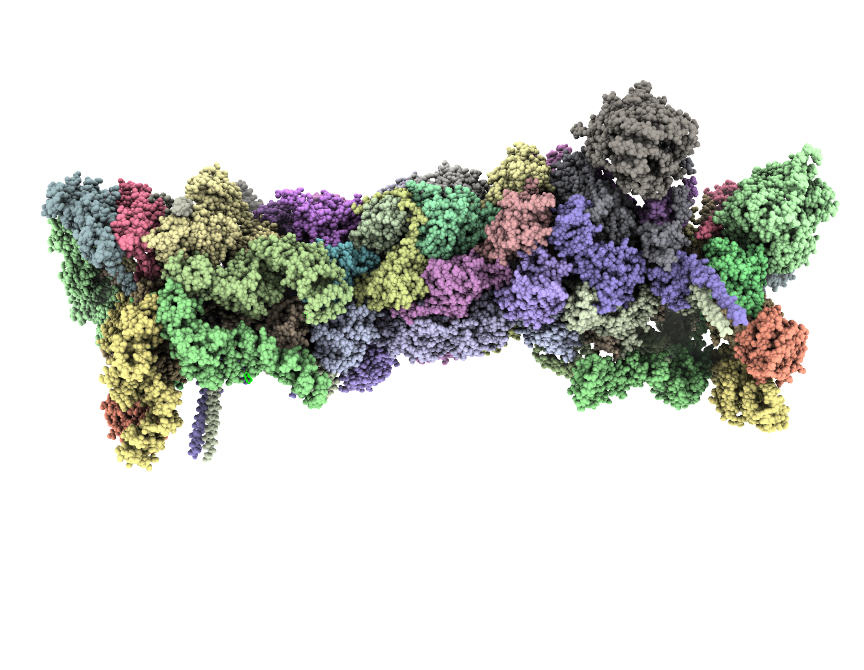
\includegraphics[width=0.3\textwidth]{figures/5gjr_structure.png}
\caption{EM structure at 3.5 {\AA} resolution of the human 26S proteasome, PDB ID: 5GJR}
\end{figure}
\begin{block}{}
  \begin{itemize}
    \item Choosing to work with the base subcomplex of the human 26S proteasome
  \end{itemize}
\end{block}
\begin{figure}
  \centering
  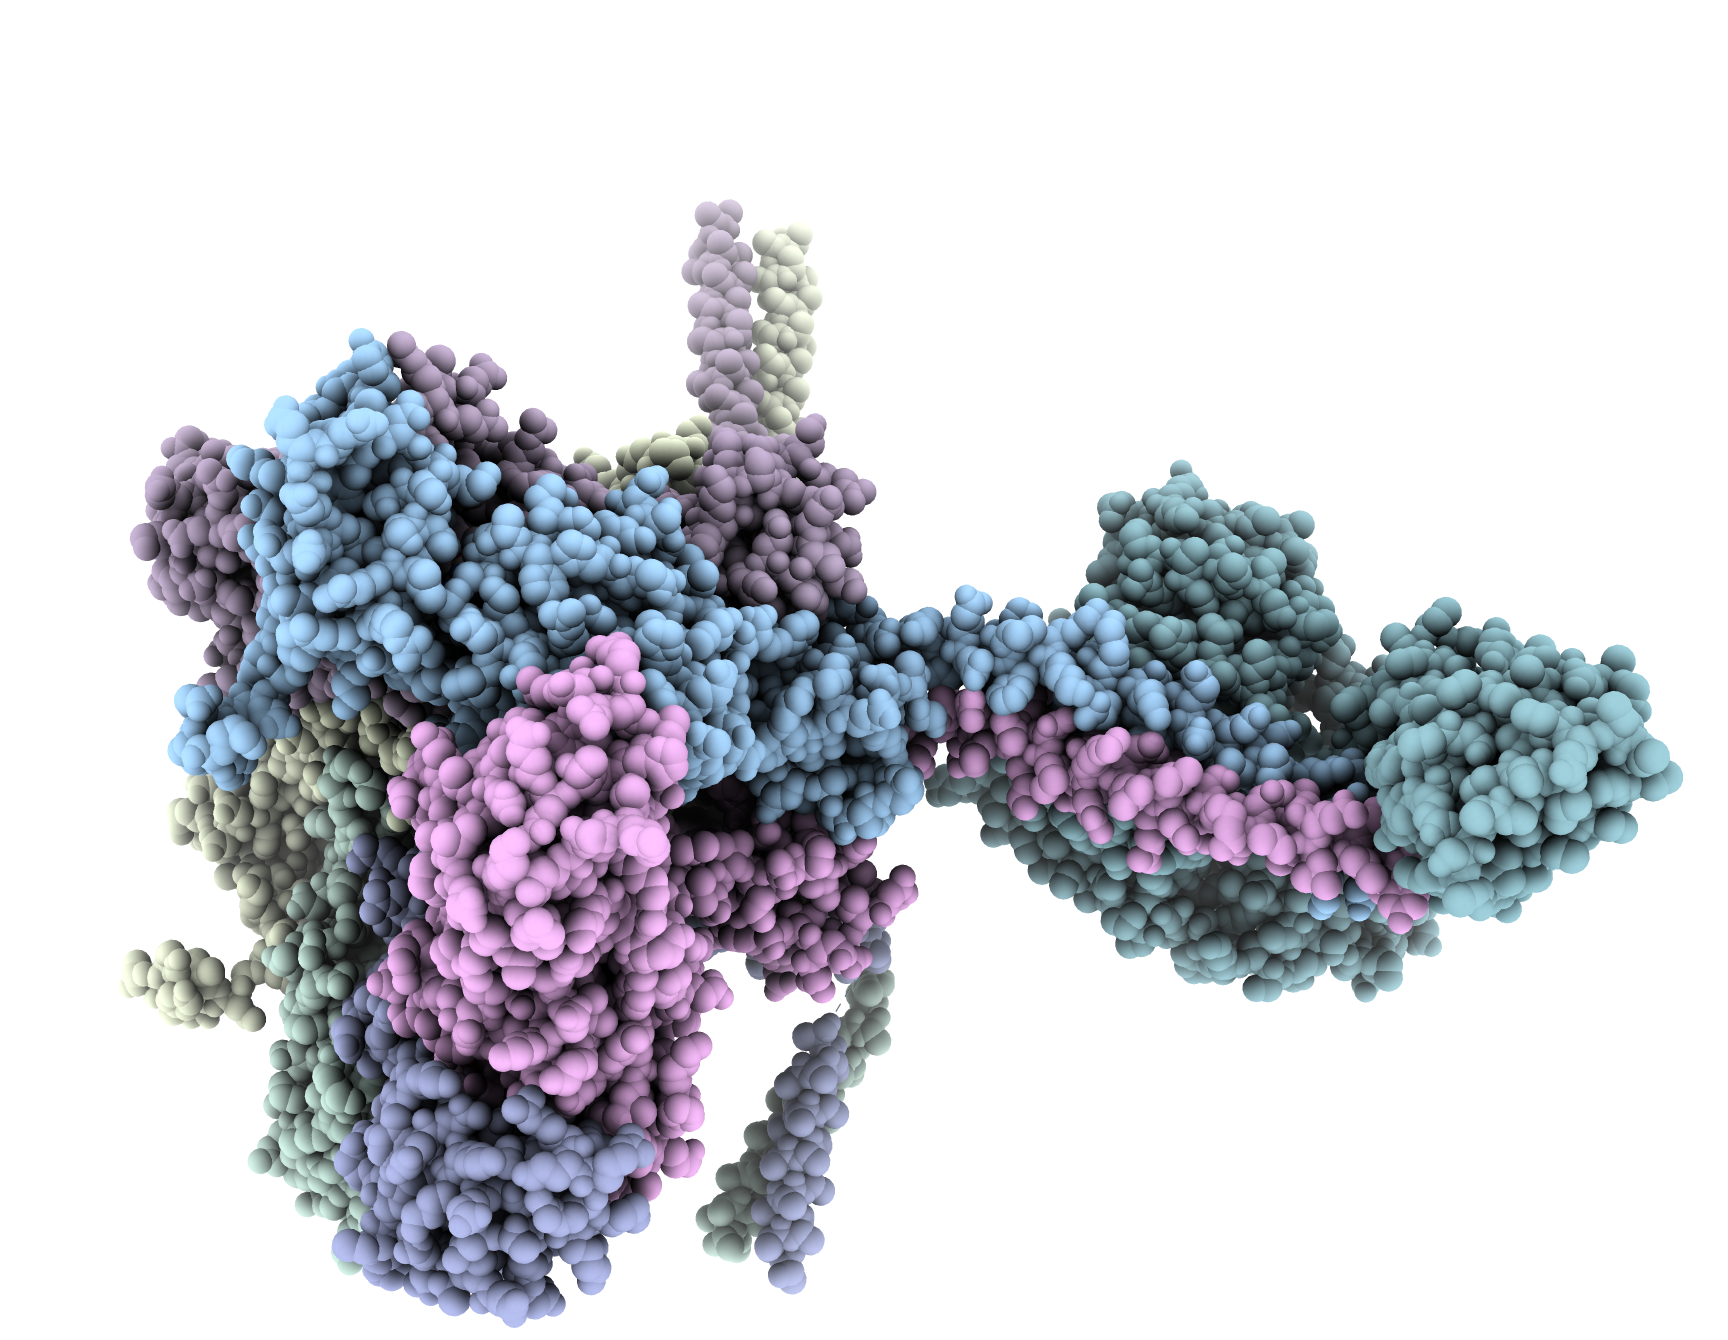
\includegraphics[width=0.3\textwidth]{figures/base_proteasome_5gjr.png}
  \caption{Base subcomplex consists of the Rpt1, Rpt2, Rpt3, Rpt4, Rpt5, Rpt6 and Rpn2 subunits
  of the human 26S proteasome}
\end{figure}
\end{frame}
%------------------------------------------------------------------------------
\begin{frame}
  \frametitle{Modeling with DSSO crosslinking data}
  \begin{figure}
  \centering
  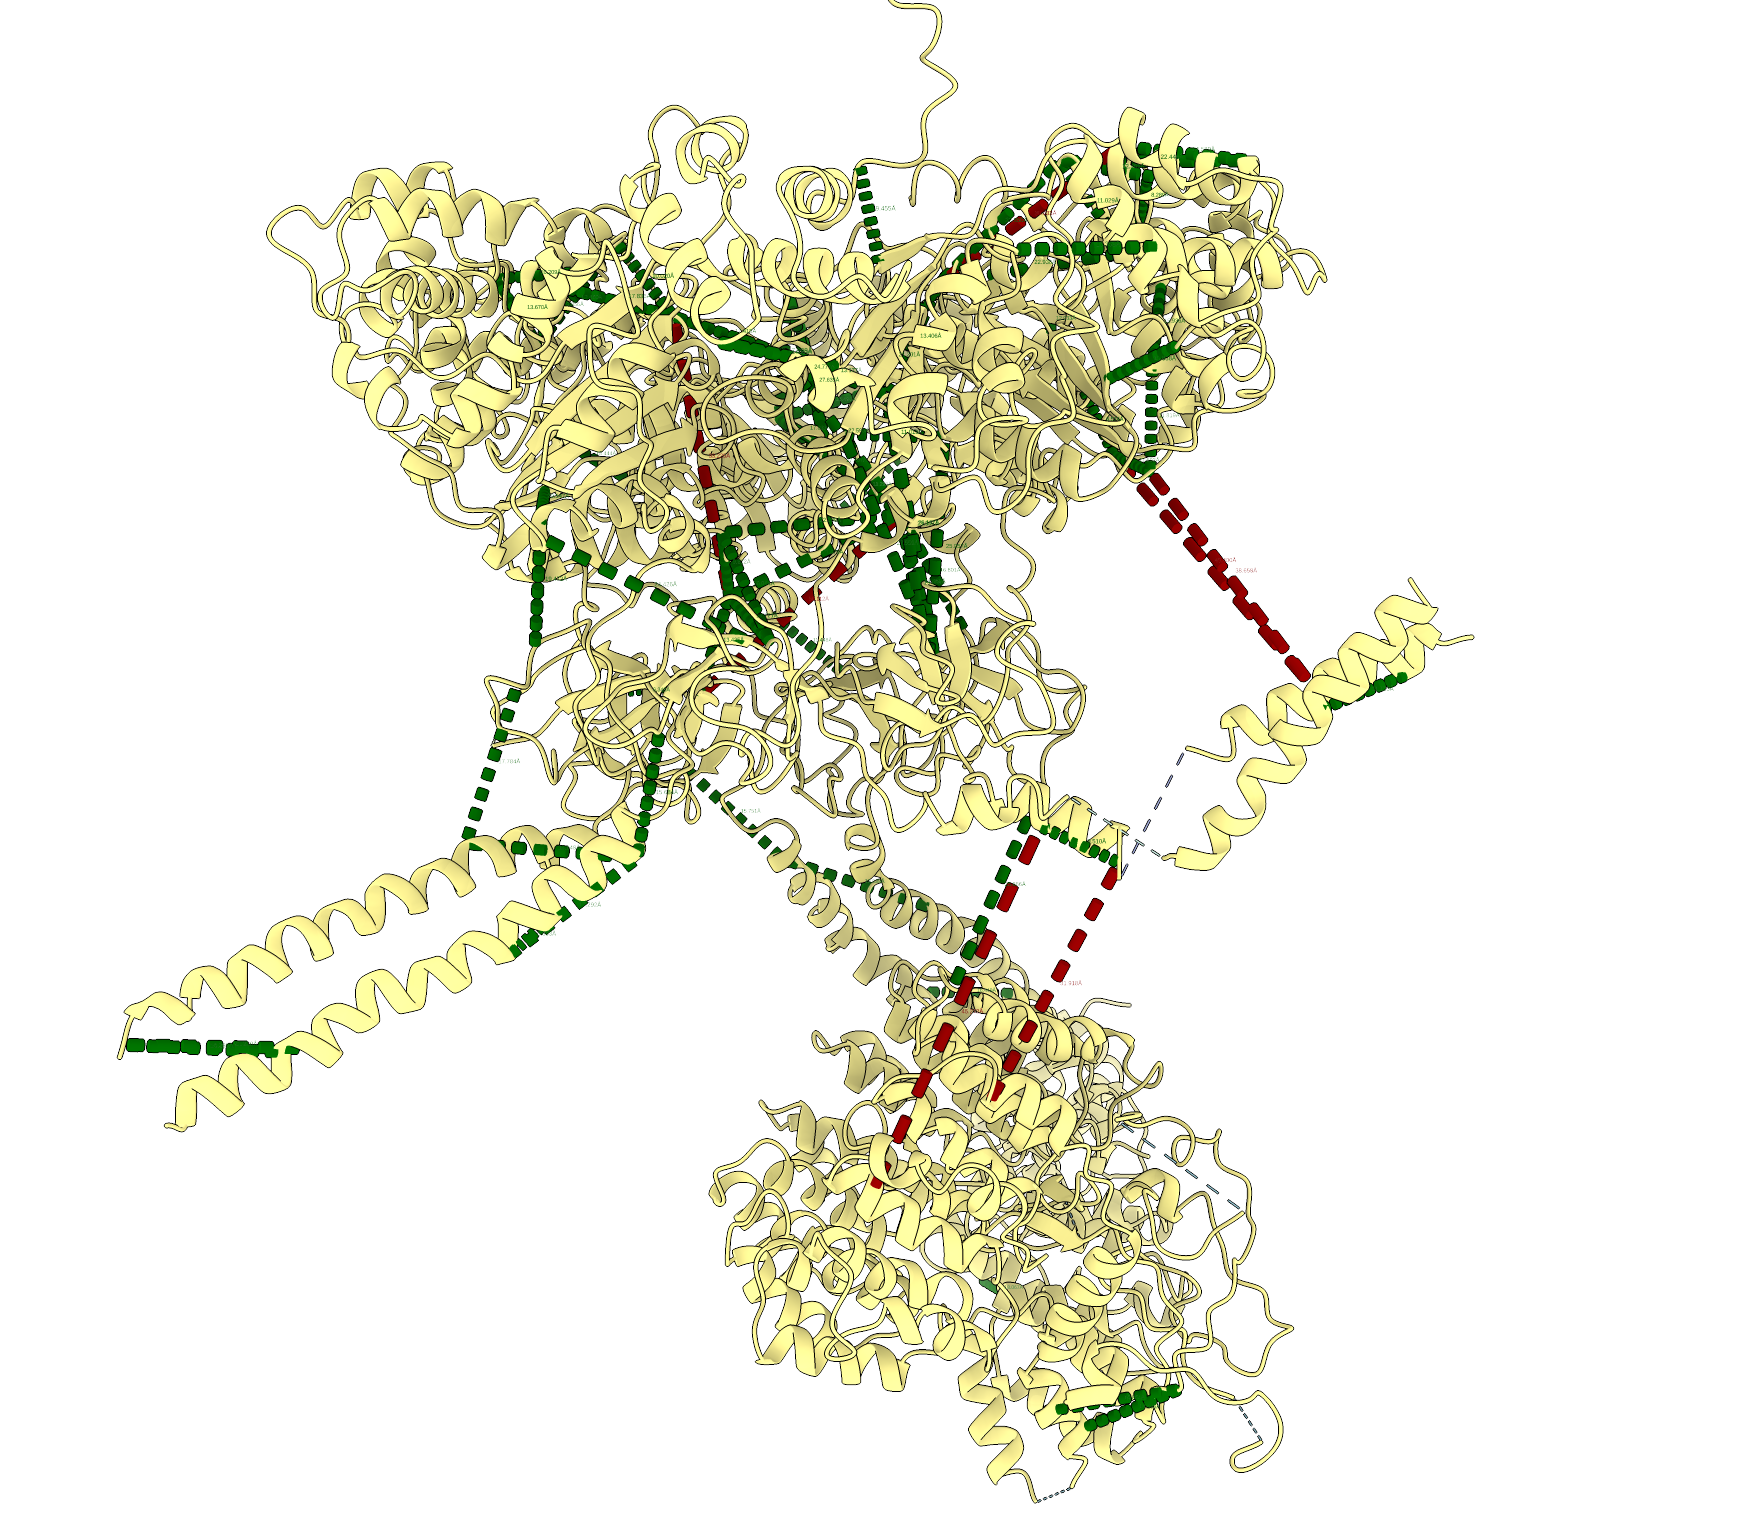
\includegraphics[width=0.4\textwidth]{figures/dsso-mapped-xls.png}
  \caption{DSSO crosslinking data mapped onto the base subcomplex, 
  there is a total of 95 identified crosslinks.}
  \end{figure}
  %
  \begin{table}
    \centering
    \caption{Modeling with DSSO XL data for the base subcomplex}
    \begin{tabular}{|c|c|}
        \hline
        Cluster precision ({\AA}) & Accuracy({\AA}) \\ \hline
        12.2 & 33 \\ \hline
    \end{tabular}
    \end{table}
    Clustering at sampling precision $20.0$ {\AA} with
    a cluster of population 28000.
  \end{frame}
%------------------------------------------------------------------------------
\begin{frame}
  \frametitle{Modeling with TSTO crosslinking data}
  \begin{minipage}{0.48\textwidth}
    \centering
    \begin{figure}
    \centering
    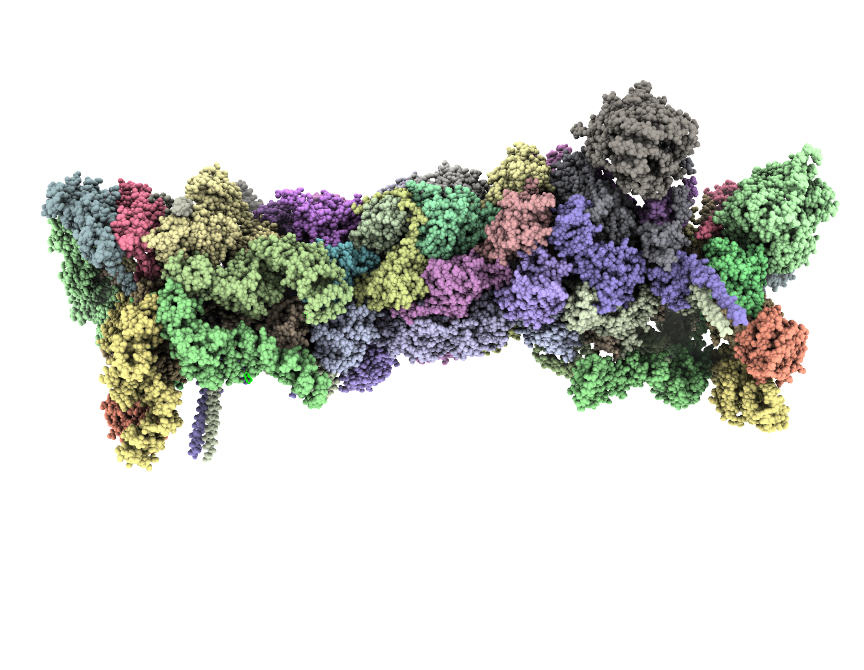
\includegraphics[width=0.5\textwidth]{figures/5gjr_structure.png}
    \caption{Structure of the human 26S proteasome, PDB ID: 5GJR}
    \end{figure}
    % a table with two rows and two columns
\begin{table}
    \centering
    \caption{Number of unique cross links}
    \begin{tabular}{|c|c|}
        \hline
        Type of XL & Number of unique XLs \\ \hline
        Tri & 35 \\ \hline
        Bi & 691 \\ \hline
    \end{tabular}
\end{table}
\end{minipage}
\hfill
\begin{minipage}{0.48\textwidth}
  \centering
  \begin{figure}
  \centering
  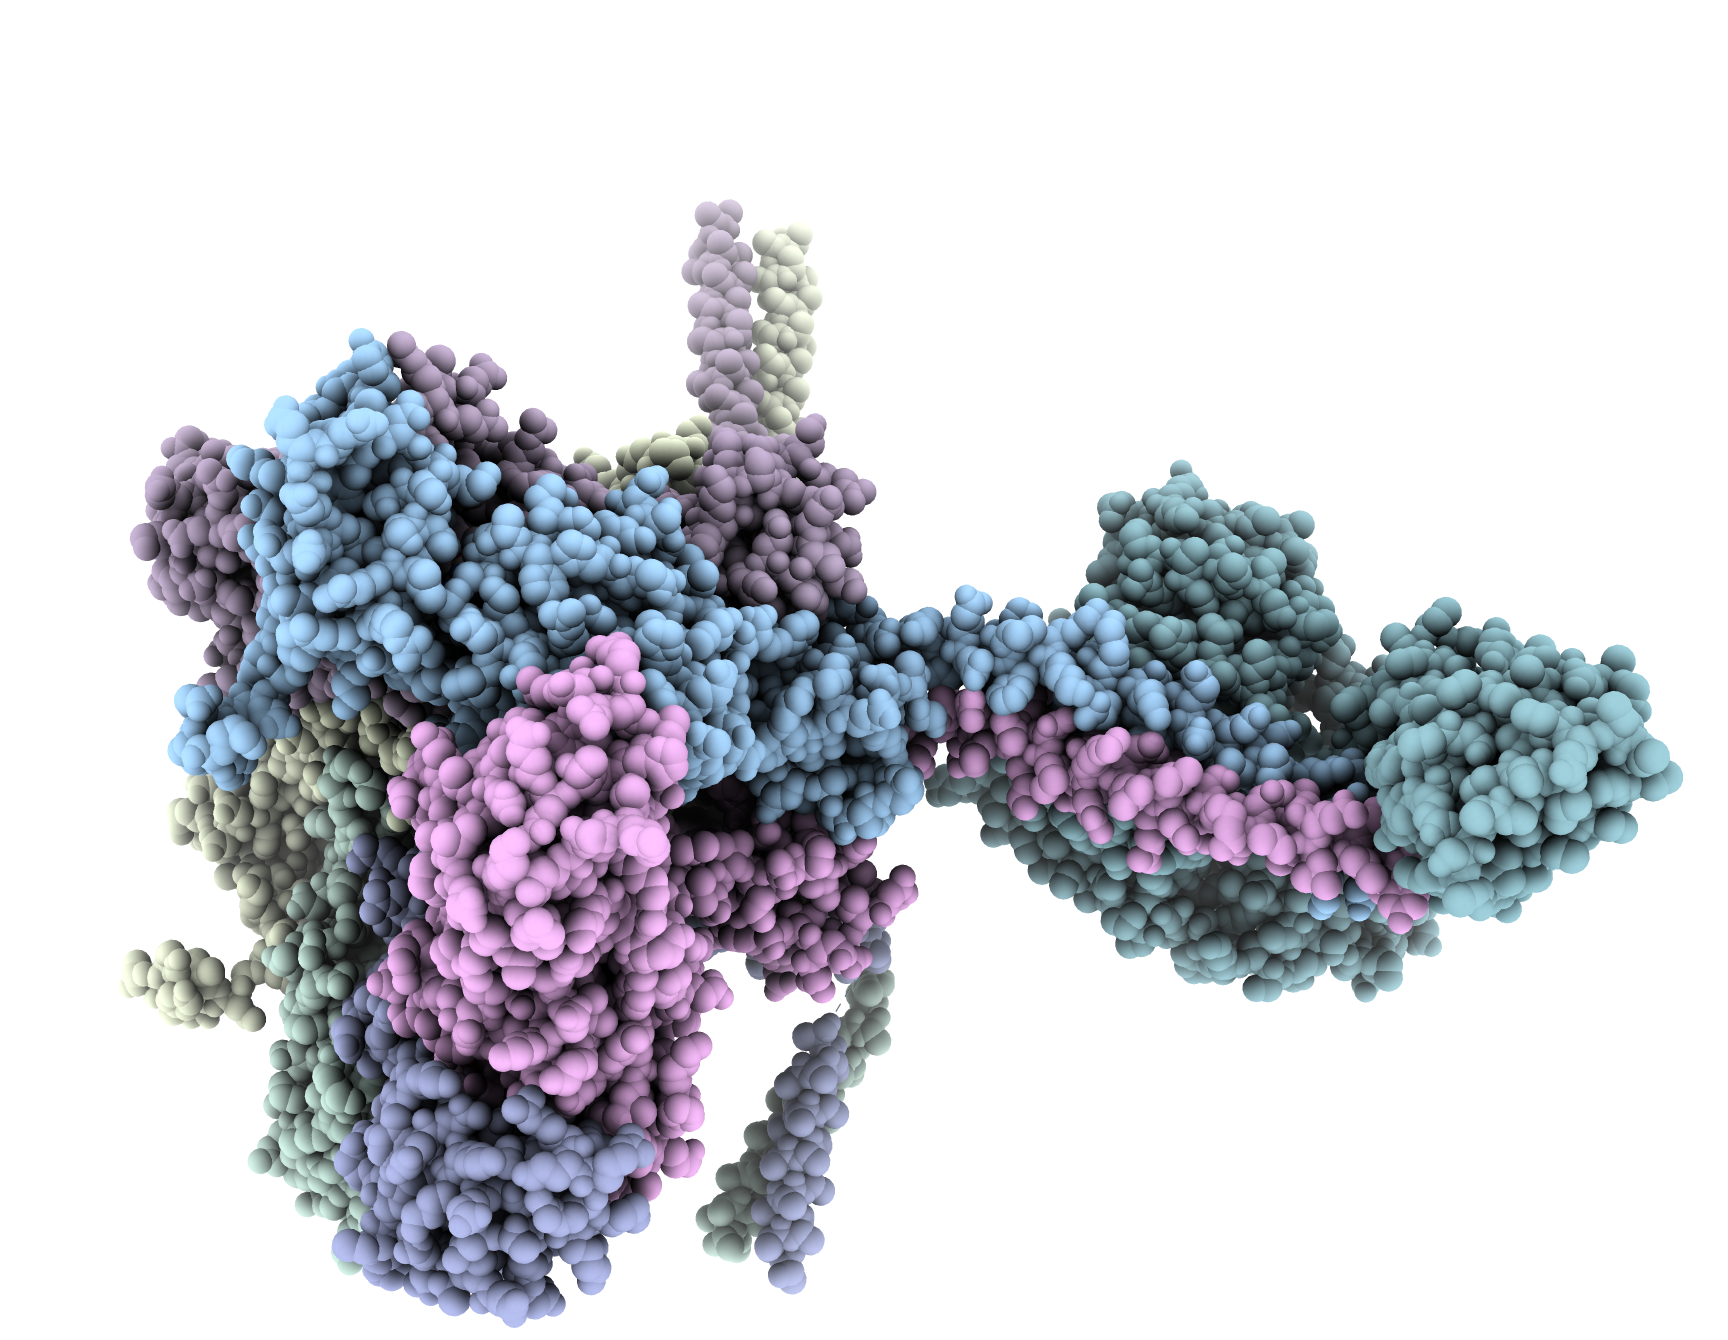
\includegraphics[width=0.5\textwidth]{figures/base_proteasome_5gjr.png}
  \caption{Base subcomplex of the human 26S proteasome}
  \end{figure}
  %
\begin{table}
  \centering
  \caption{Number of unique cross links}
  \begin{tabular}{|c|c|}
      \hline
      Type of XL & Number of unique XLs \\ \hline
      Tri & 14 \\ \hline
      Bi & 164 \\ \hline
  \end{tabular}
\end{table}
\end{minipage}
\end{frame}
%------------------------------------------------------------------------------
\begin{frame}
\frametitle{Comparison of the bi- and tri-functional XL datasets}
\begin{block}{}
\begin{itemize}
  \item Only bifunctional set ($n(bi) = 164$)
  \item Only trifunctional set ($n(tri)= 42$)
  \item bifunctional + trifunctional set ($n(bi) + n(tri) = 206$)
  \item n($bi \cup tri) = n(bi) + n(tri) - n(bi\cap tri) = 186$
\end{itemize}
\end{block}
    \begin{figure}
      \centering
      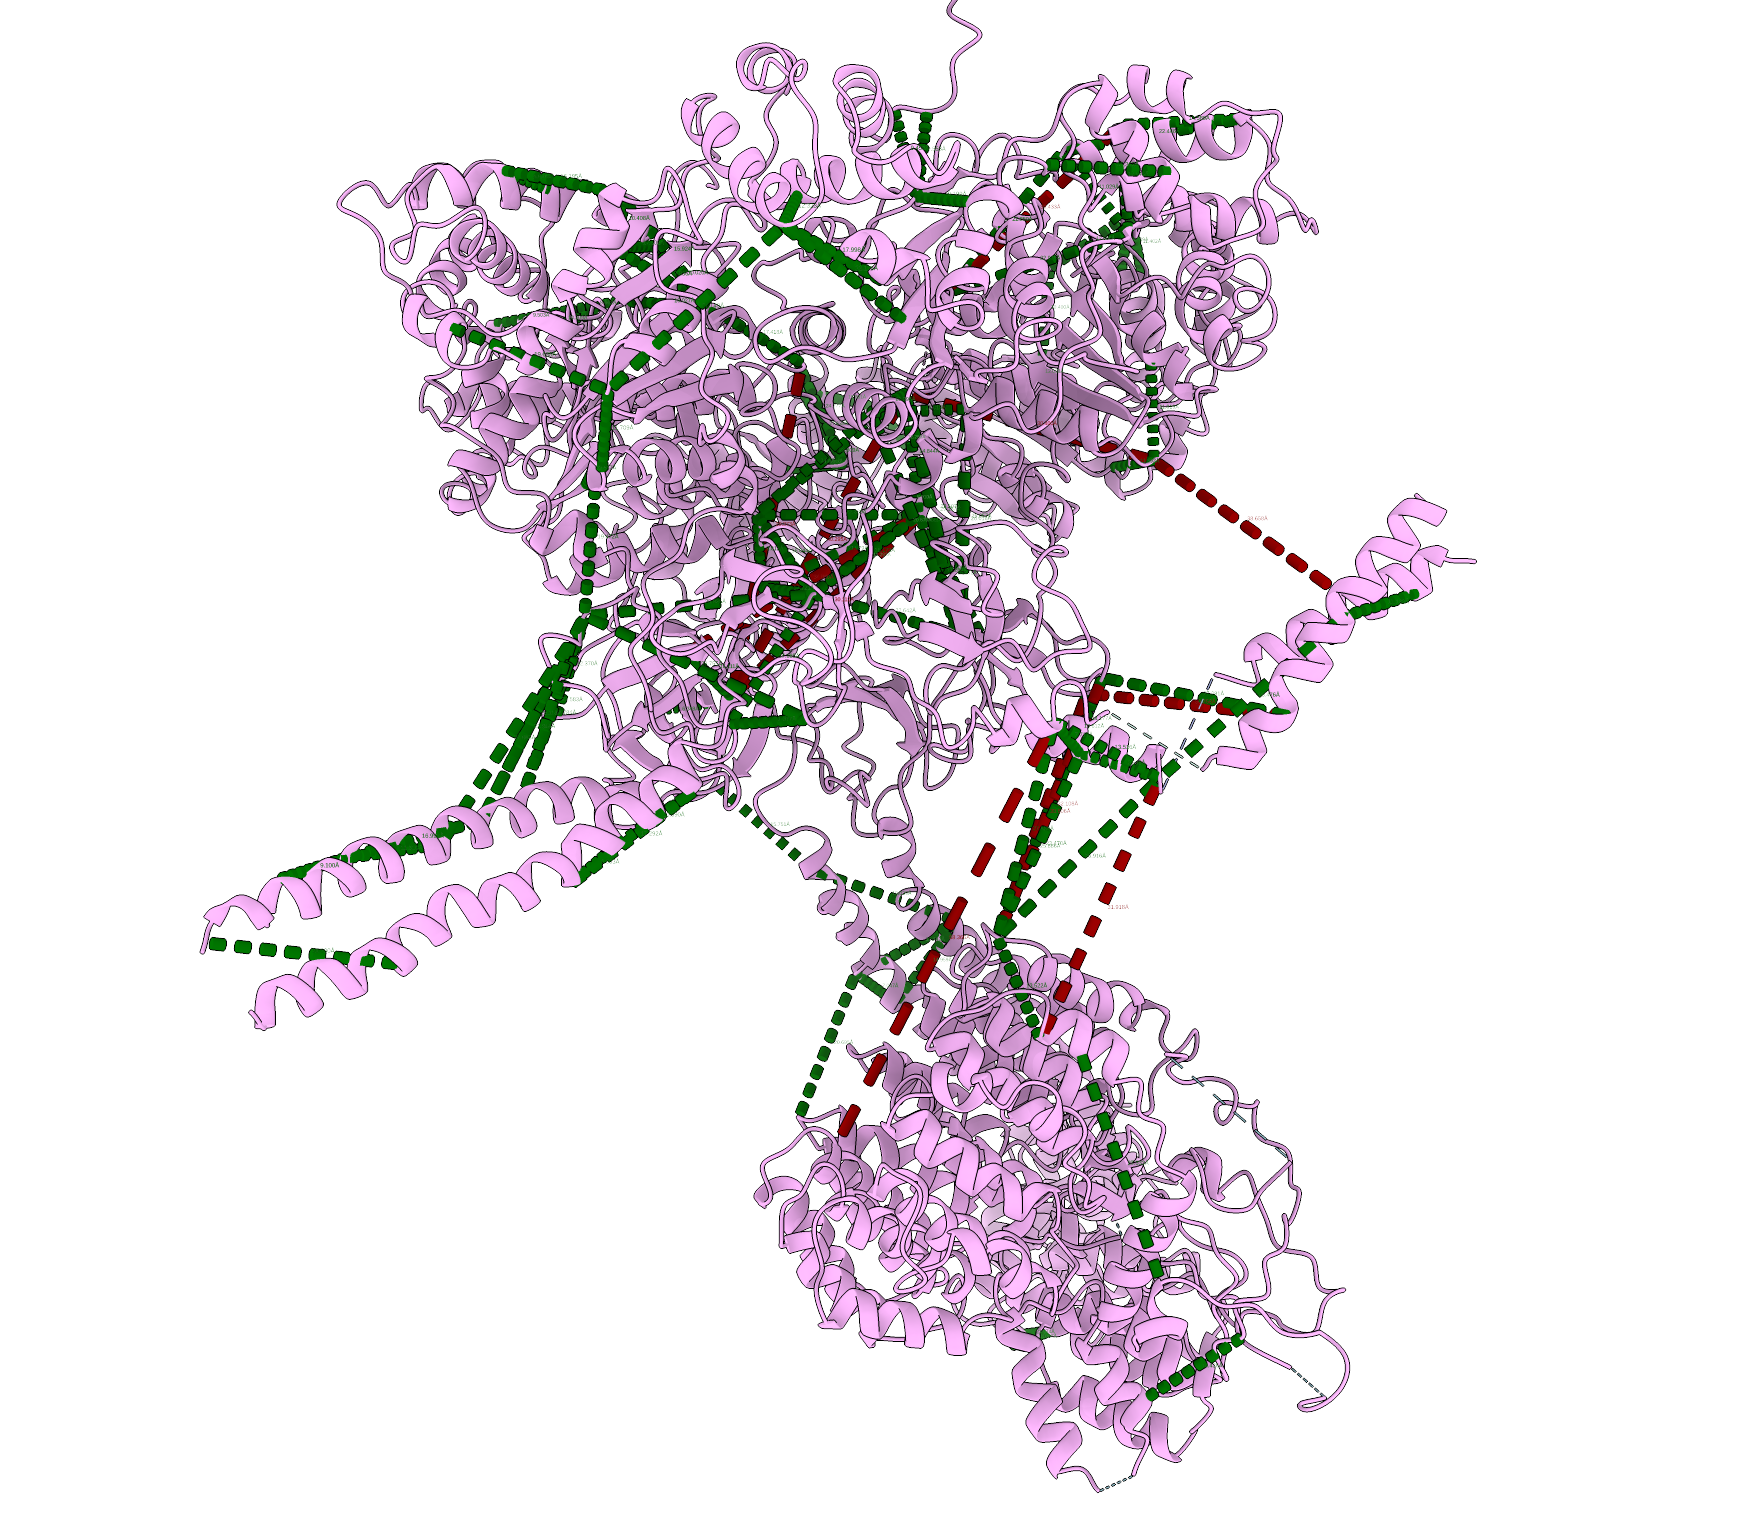
\includegraphics[width=0.43\textwidth]{figures/only-doubles.png}
      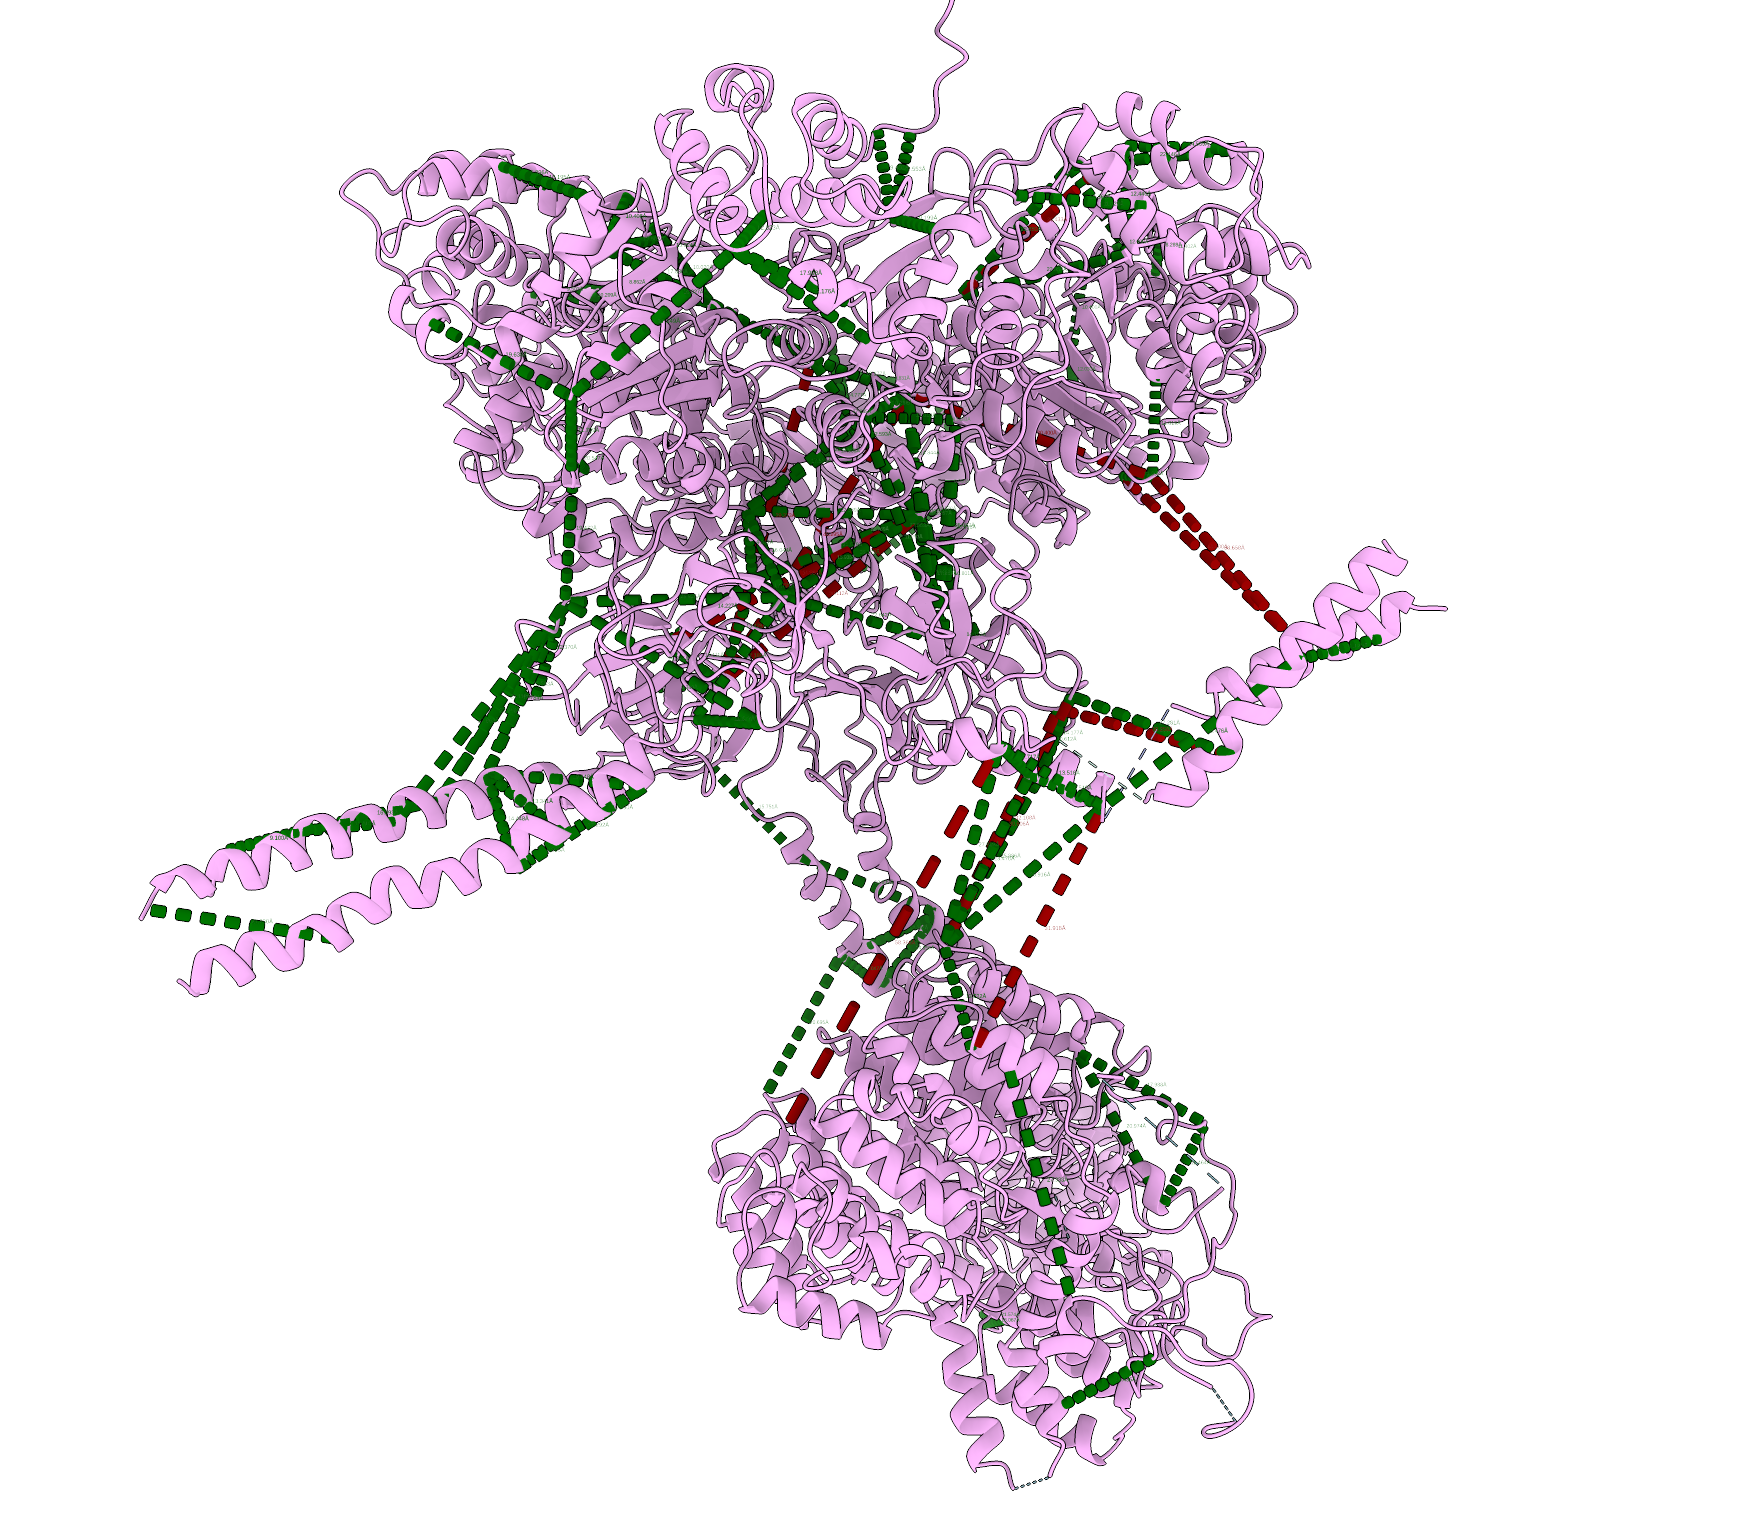
\includegraphics[width=0.43\textwidth]{figures/removed-doubles-plus-triples.png}
      \caption{$n(bi) = 164$ (left) and n($bi \cup tri = 186$) (right) set of cross links mapped onto the base subcomplex}
    \end{figure}
\end{frame}
%------------------------------------------------------------------------------
\begin{frame}
\frametitle{Results}
\begin{table}
  \centering
  \caption{Comparison of the double and triple XL datasets}
  \begin{tabular}{|c|c|c|c|}
      \hline
                                   & Samp. precision ({\AA}) &  Clust. precision & Accuracy\\ \hline
      bifunctional ($n(bi) = 164$) & 4.42   & 3.335 & 14.43 \\\hline
      $n(bi) + n(tri) = 206$       & 5.58   & 3.666 & \\ \hline
      n($bi \cup tri) = 186$       & 10.68  & 7.388 &  16.09 \\\hline
  \end{tabular}
\end{table}
Clustering at sampling precision $6.0$ {\AA}
\begin{table}
  \centering
  \caption{Comparison of the double and triple XL datasets}
  \begin{tabular}{|c|c|c|c|}
      \hline
                                   &  Clust. precision & Accuracy\\ \hline
      bifunctional ($n(bi) = 164$) &  3.755 & 14.42\\ \hline
      n($bi \cup tri) = 186$       &  4.118 & 16.06\\ \hline
  \end{tabular}
\end{table}
\end{frame}
%------------------------------------------------------------------------------
\begin{frame}
  \frametitle{Distance analysis for the triangular XL restraint}
  \begin{figure}
    \centering
    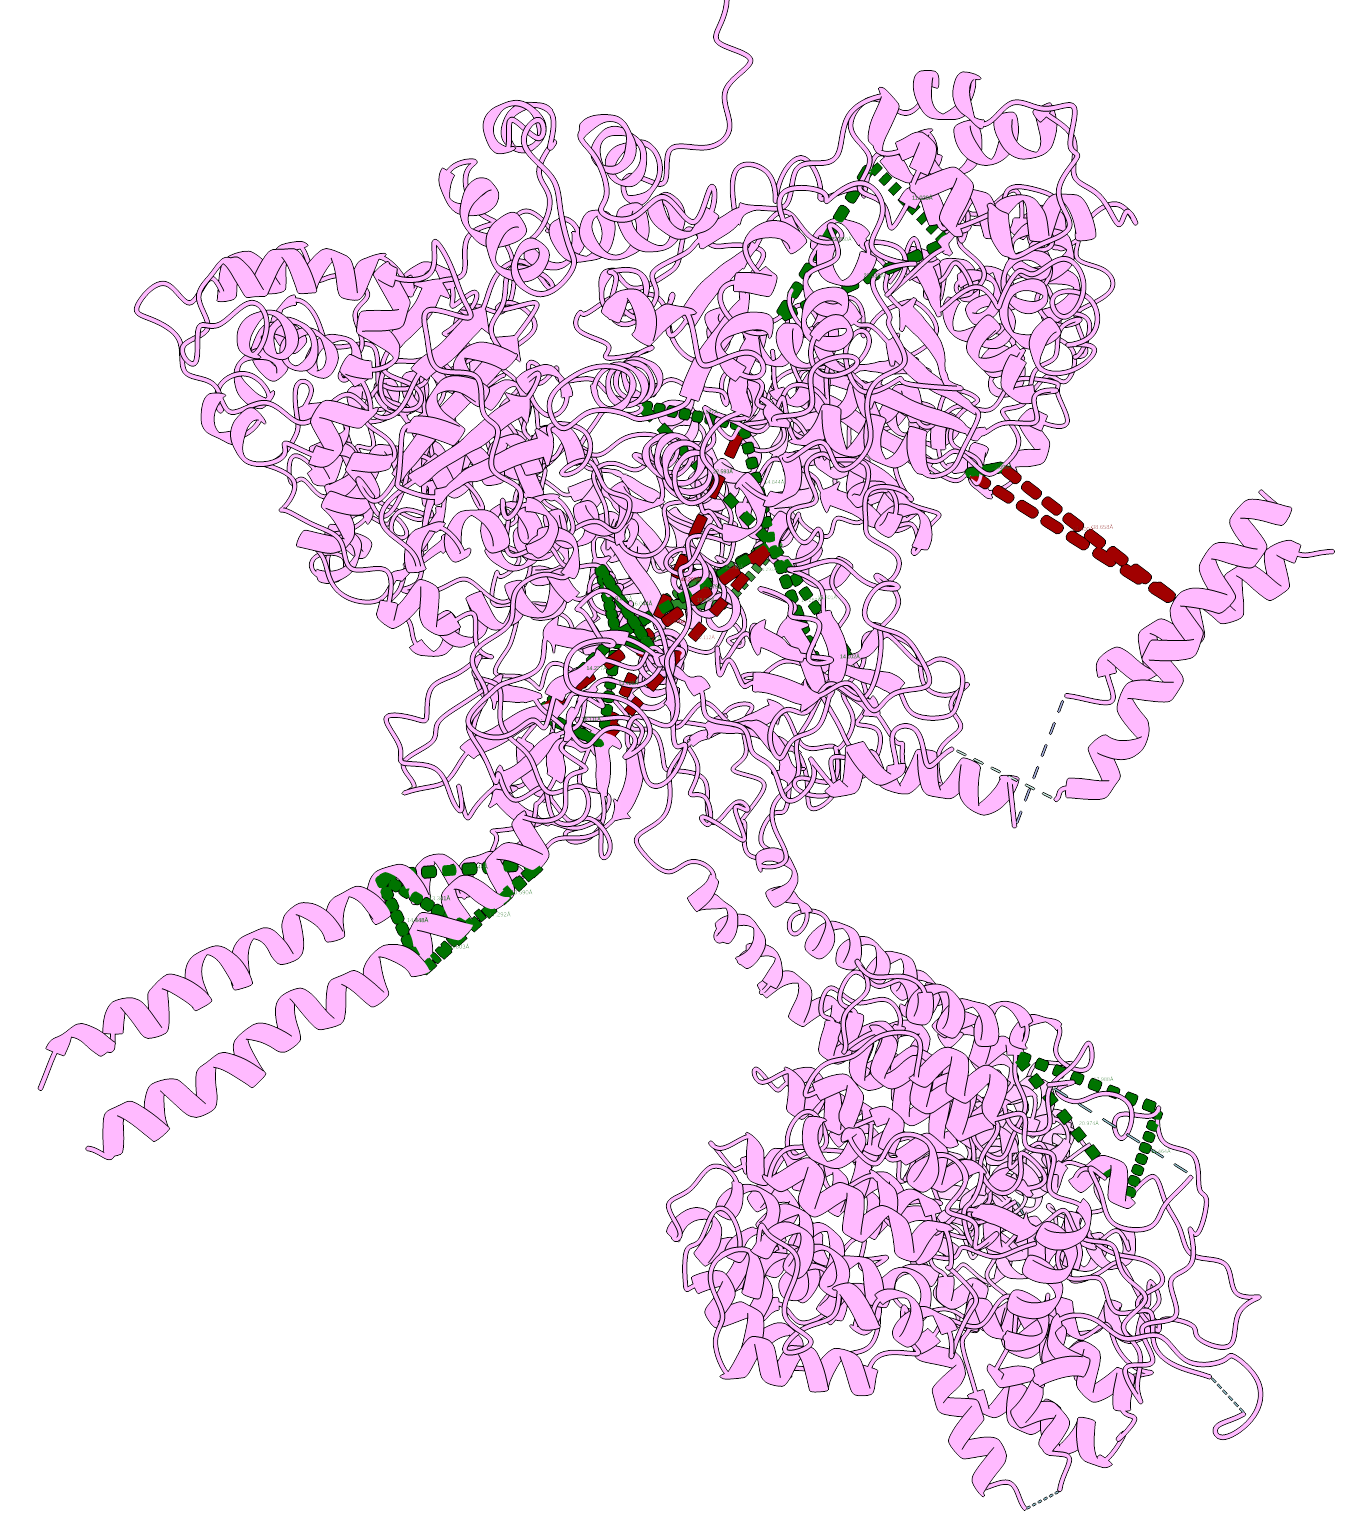
\includegraphics[width=0.3\textwidth]{test-figures/exp-triples.png}
    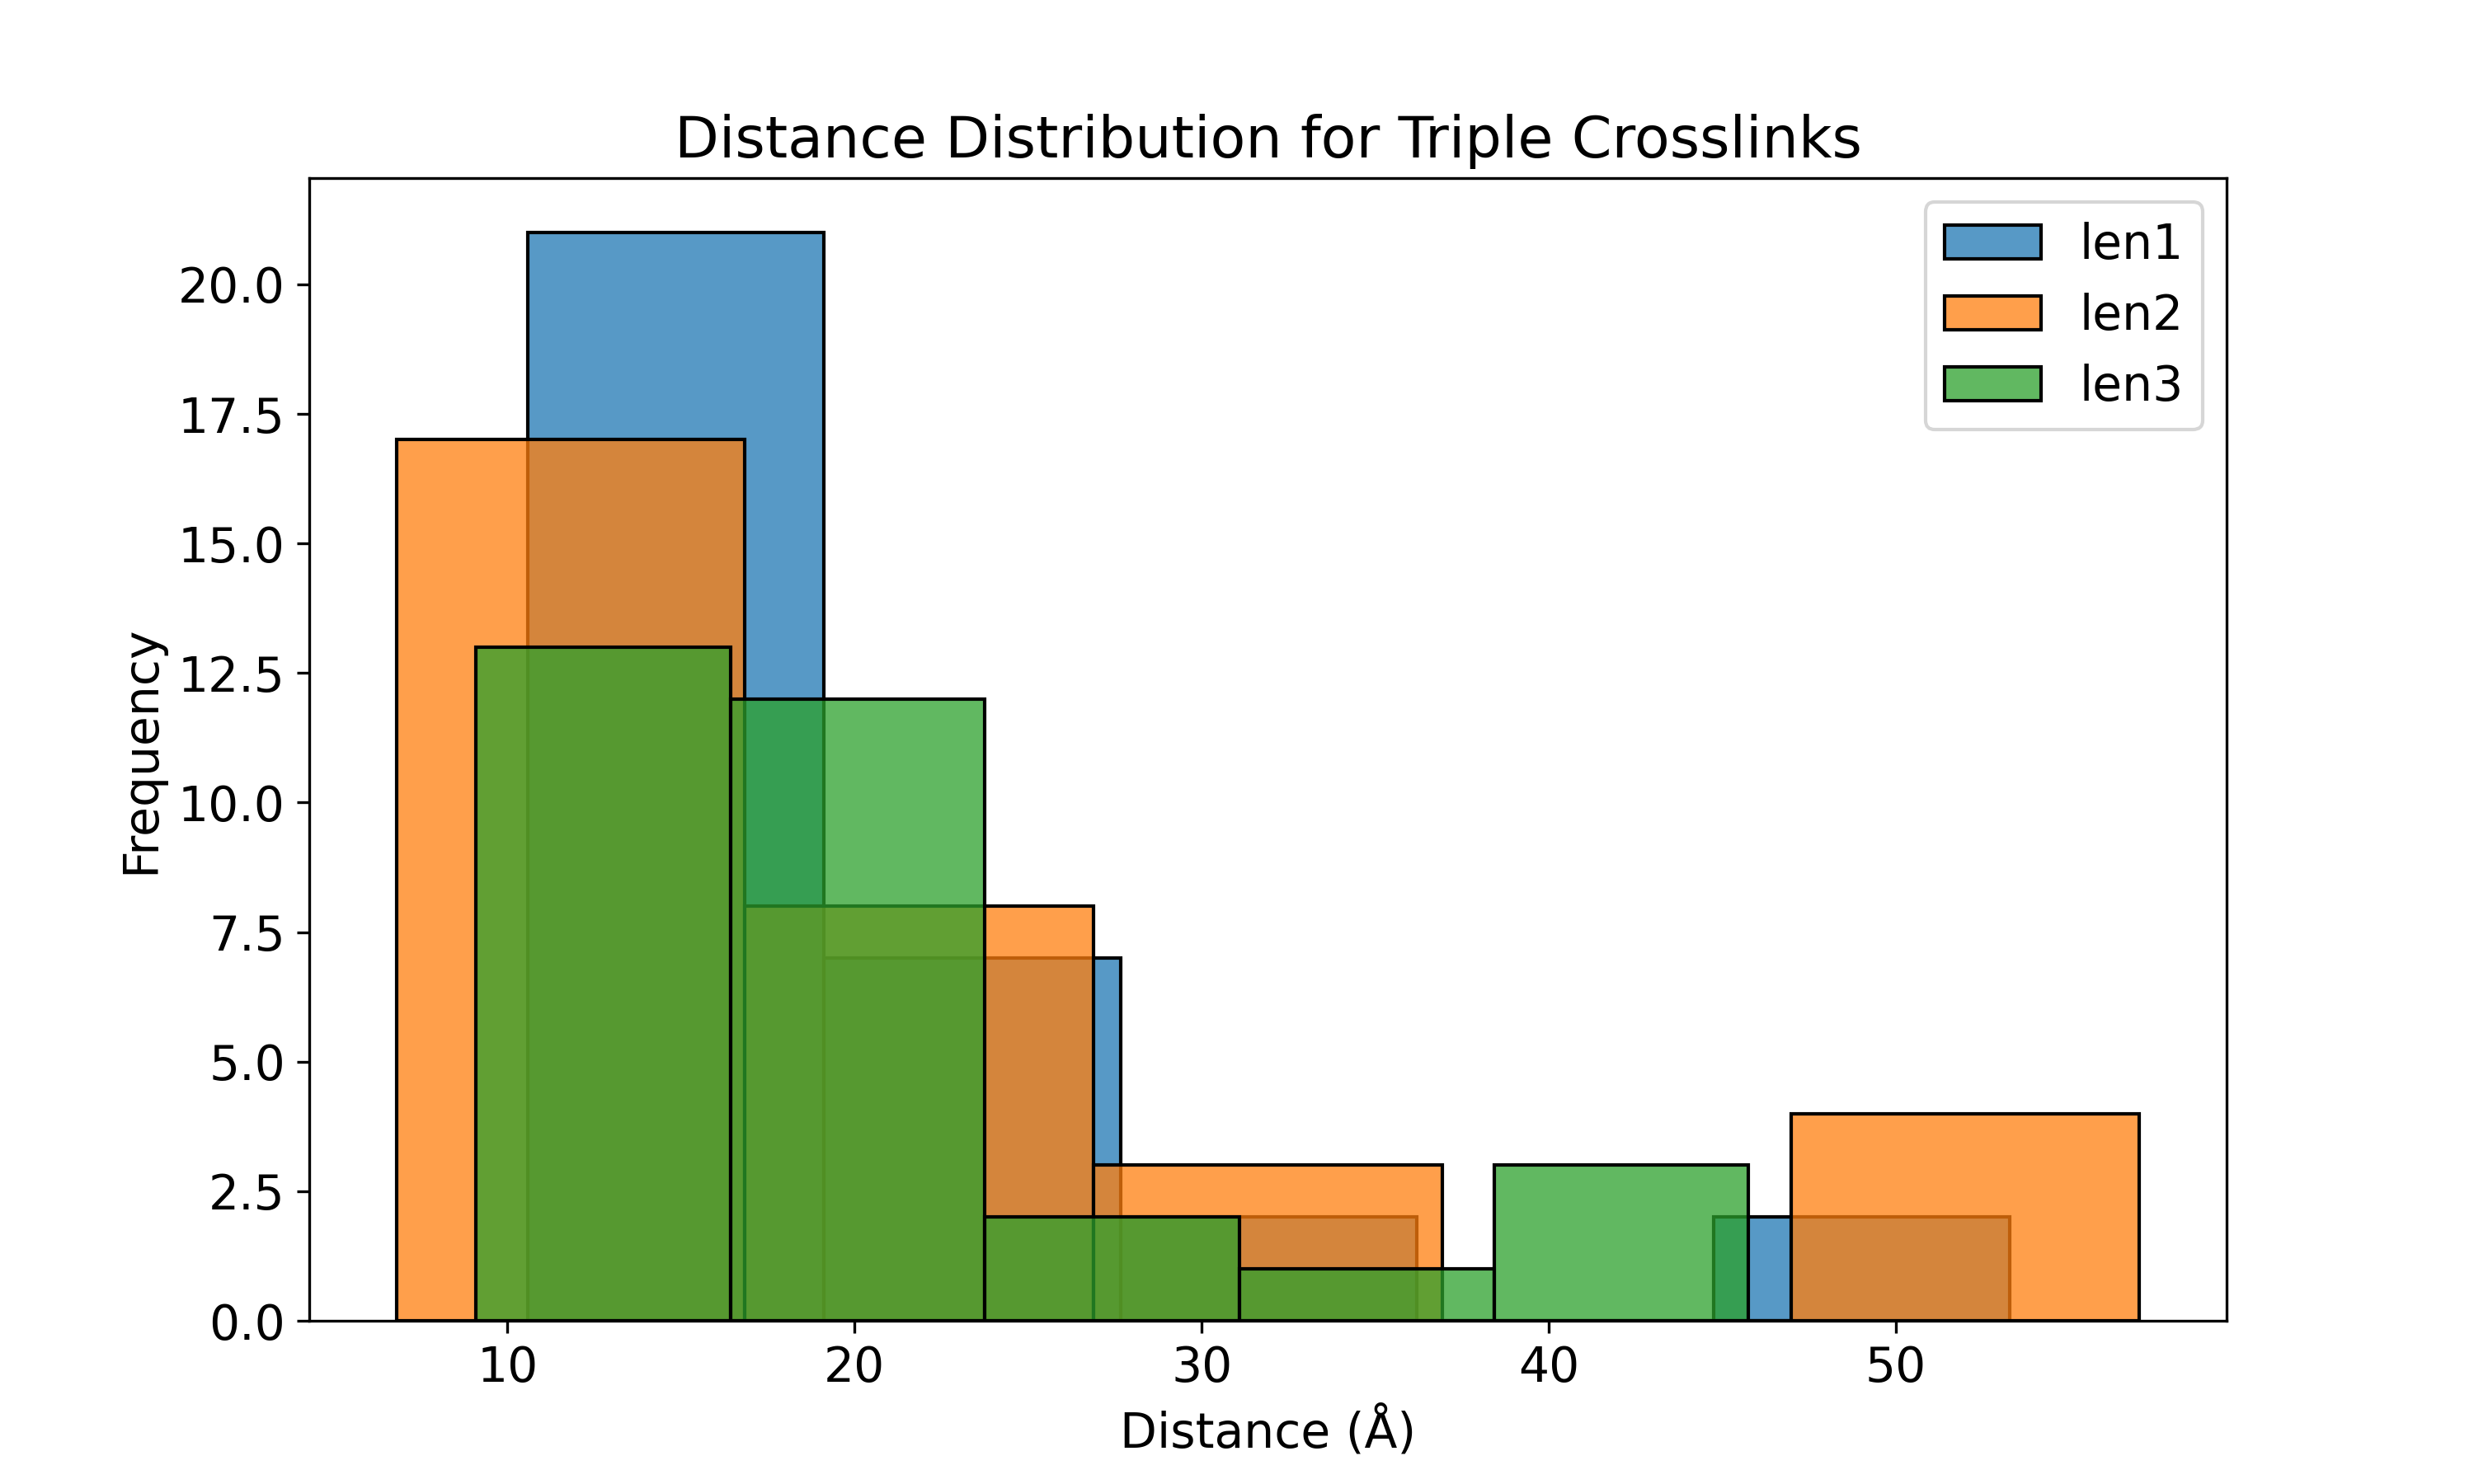
\includegraphics[width=0.45\textwidth]{test-figures/tri-distribution.png}
    \caption{Experimental trifunctional XLs mapped onto the pdb structure (left), and the distance distribution on the right, with
    mean = 19.8 {\AA}, 21.9 {\AA}, 20.0 {\AA} and std dev = 10.0 {\AA}, 14.0 {\AA}, 9.0 {\AA}, for the three pairs, respectively.}
    \end{figure}
\end{frame}
%------------------------------------------------------------------------------
\begin{frame}
  \frametitle{TSTO crosslinking data distance distribution}
  \begin{figure}
    \centering
    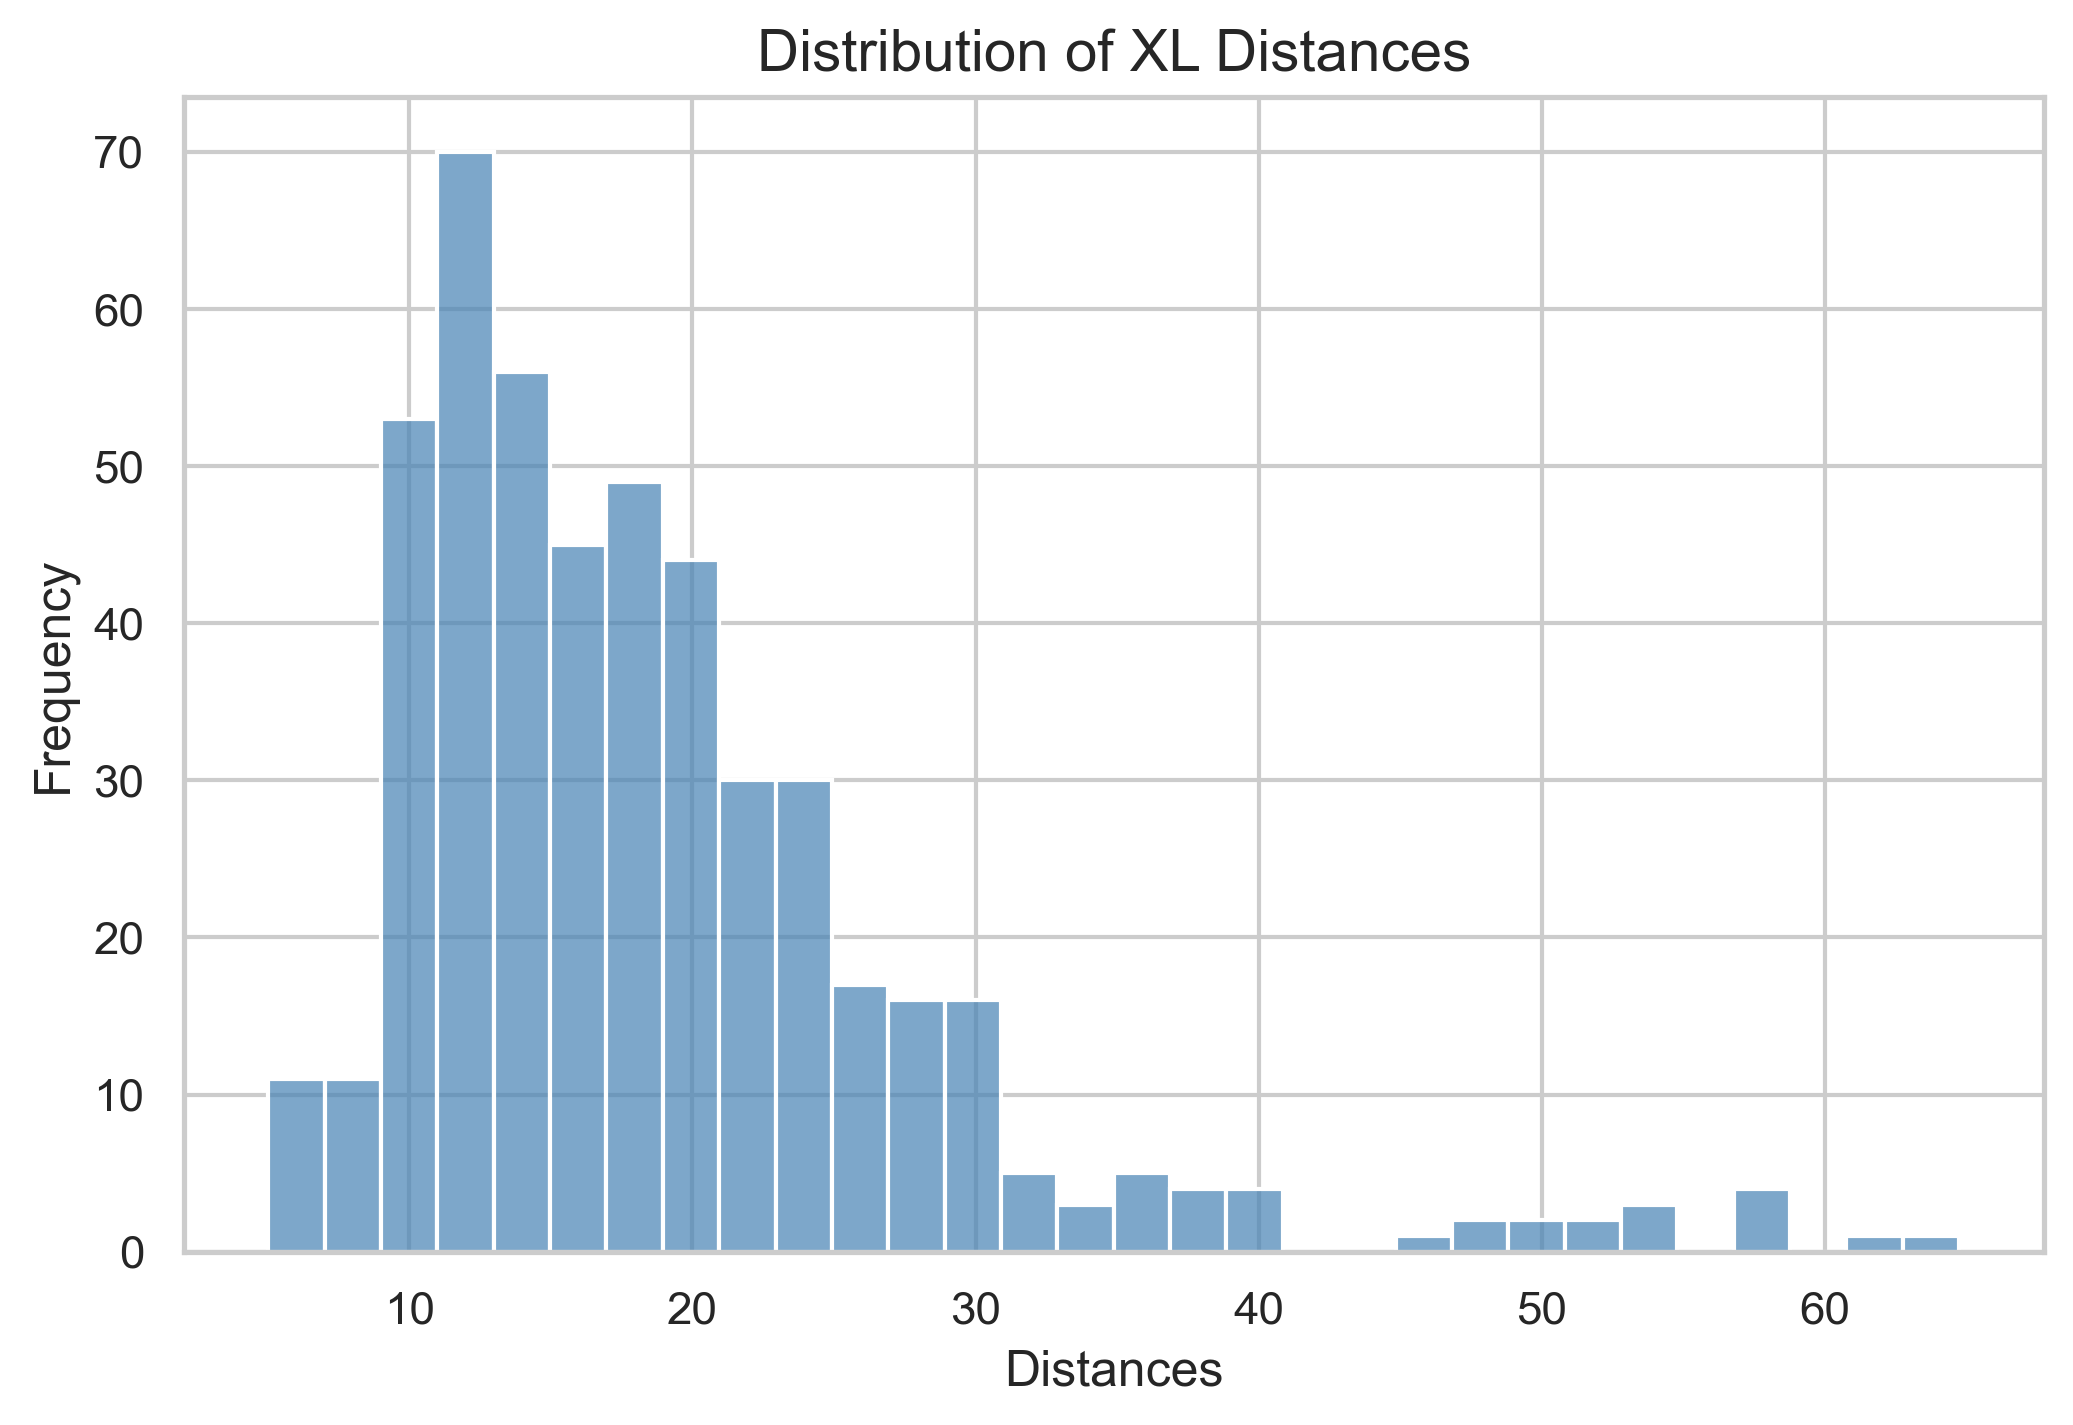
\includegraphics[scale=0.3]{test-figures/distance_histogram.png}
    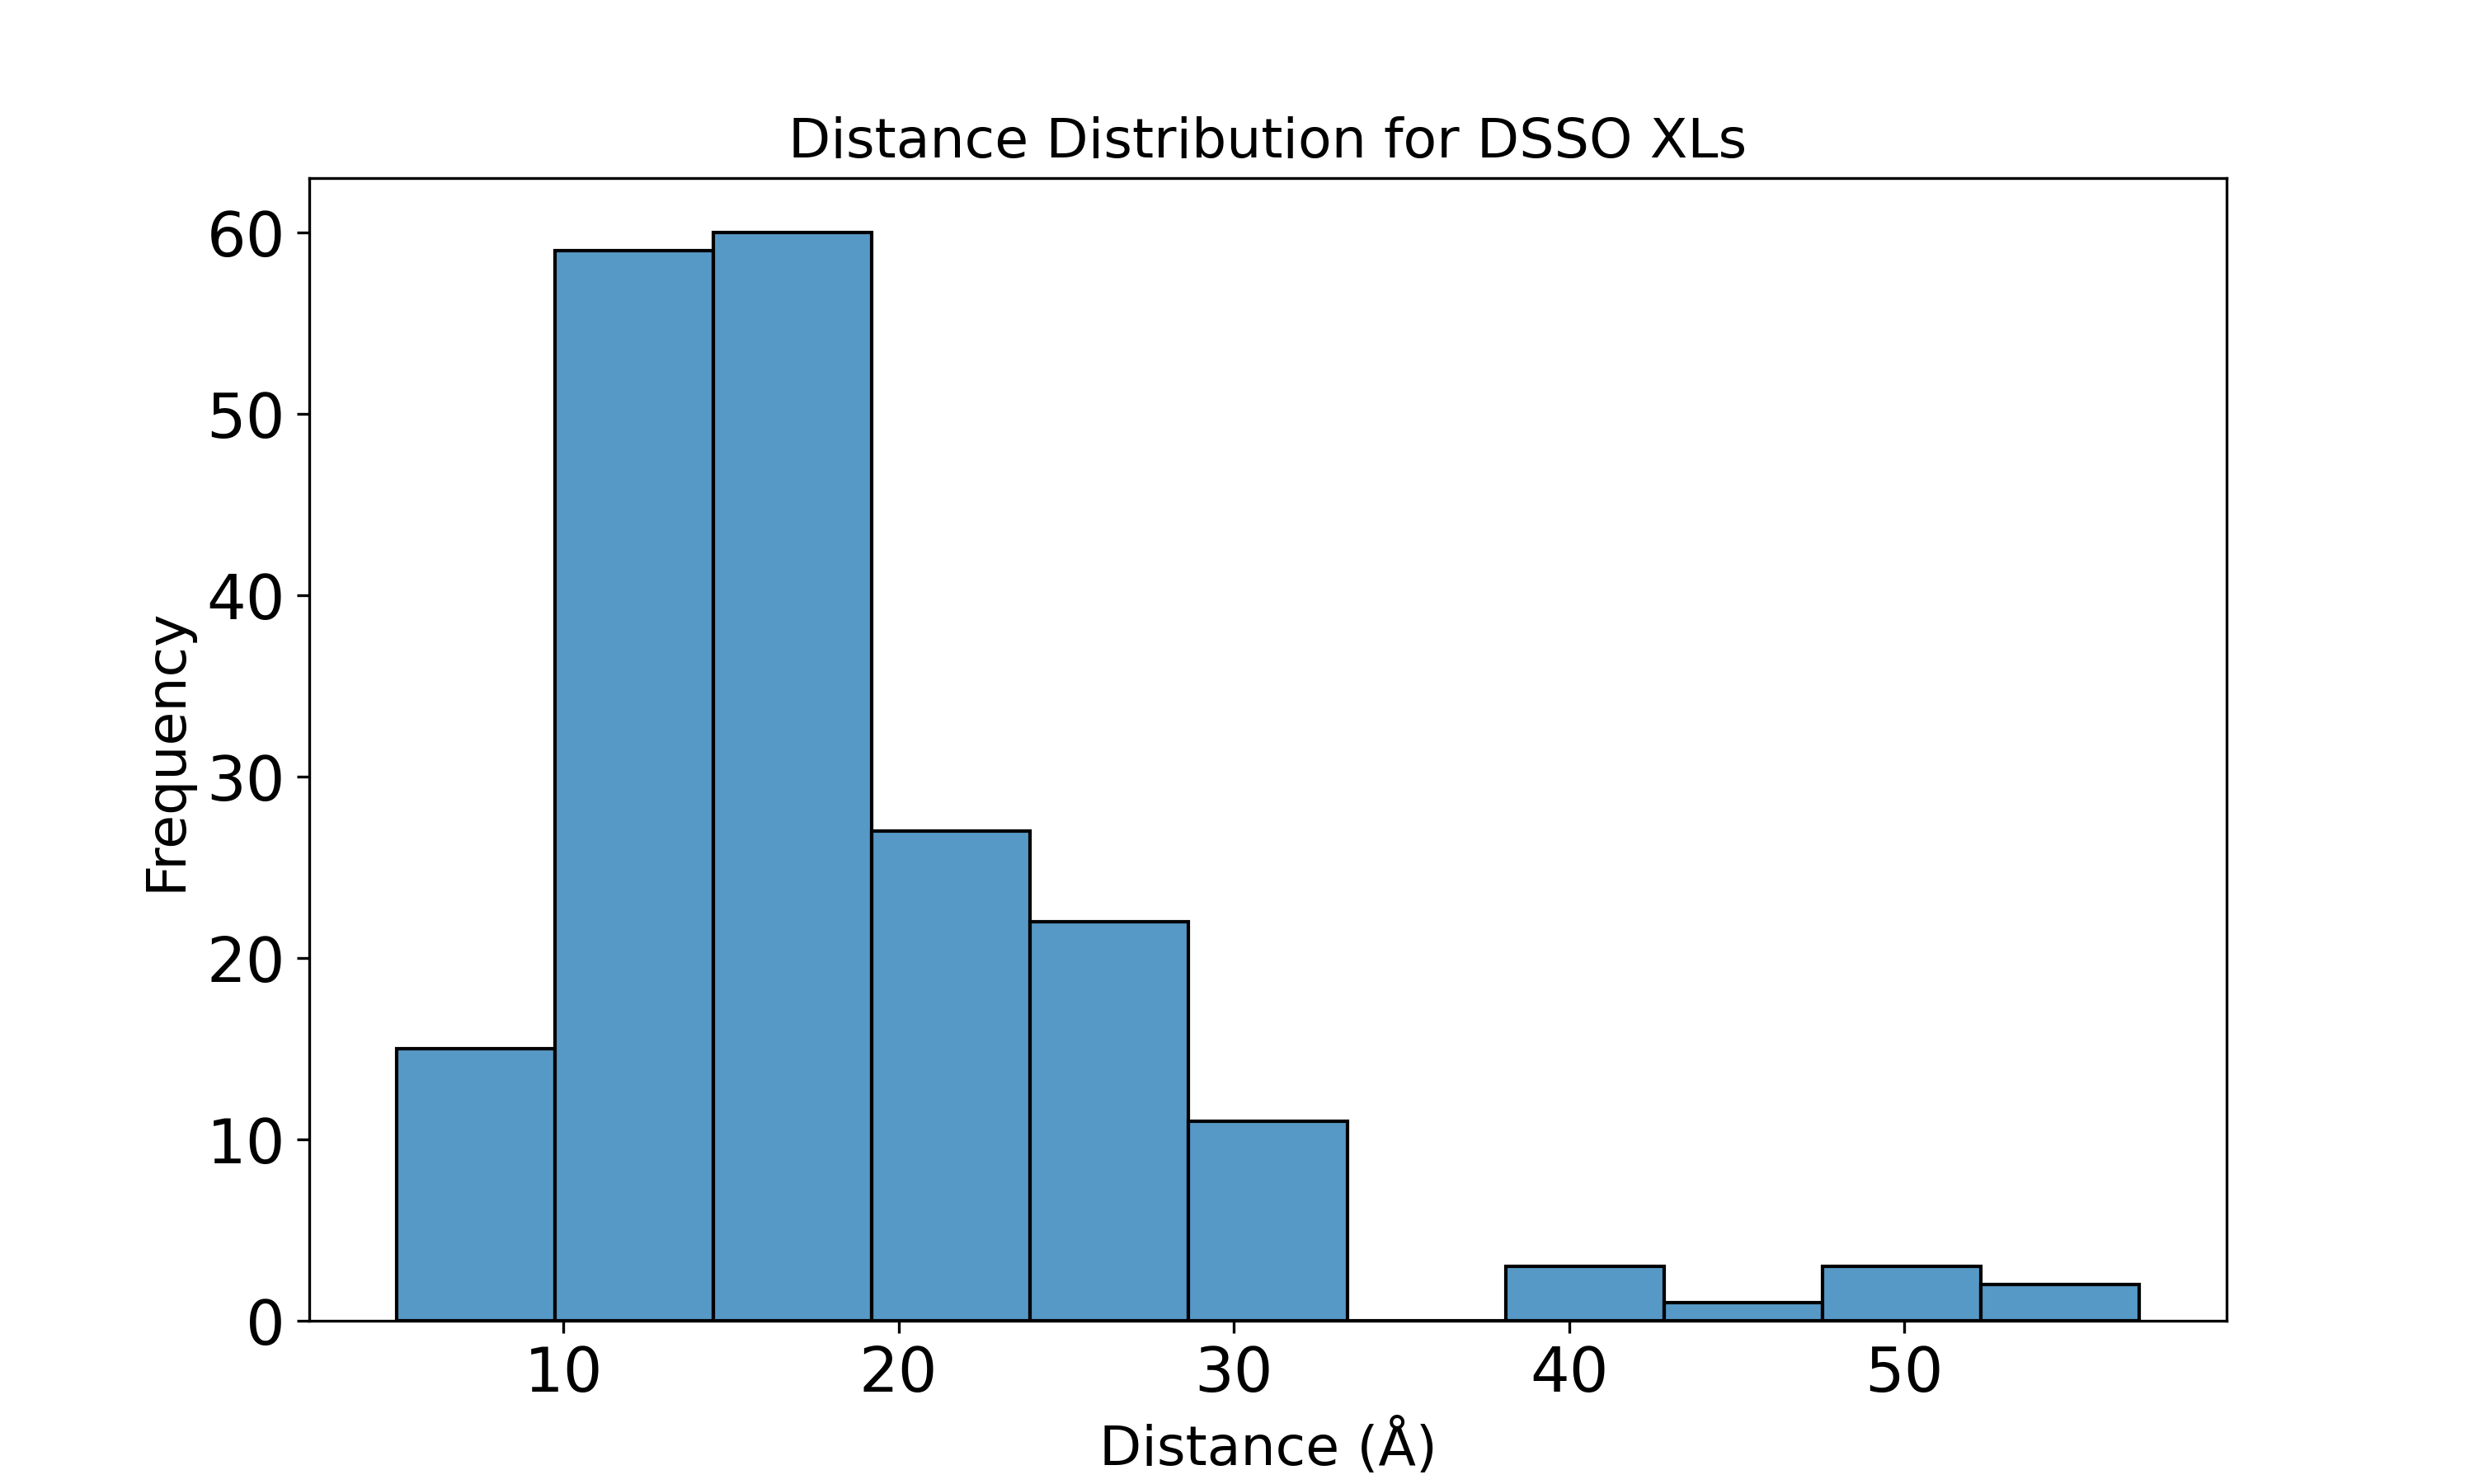
\includegraphics[scale=0.2]{test-figures/dsso_distances.png}
  \end{figure}
  \end{frame}
%------------------------------------------------------------------------------
\begin{frame}
\frametitle{Optimizing the crosslinker length}
\begin{block}{}
\begin{itemize}
  \item use the proteins Rpt2, Rpt4, Rpt5, Rpt6 for the simulations
  \item There are 4 trifunctional cross links between these proteins
  \item The cross linker length is varied from 11 to 21 {\AA}
  \item The 4 cross links are made into 12 pairs of regular crosslinks and used to get the reference distance distributions
\end{itemize}
\end{block}
\begin{figure}
\centering
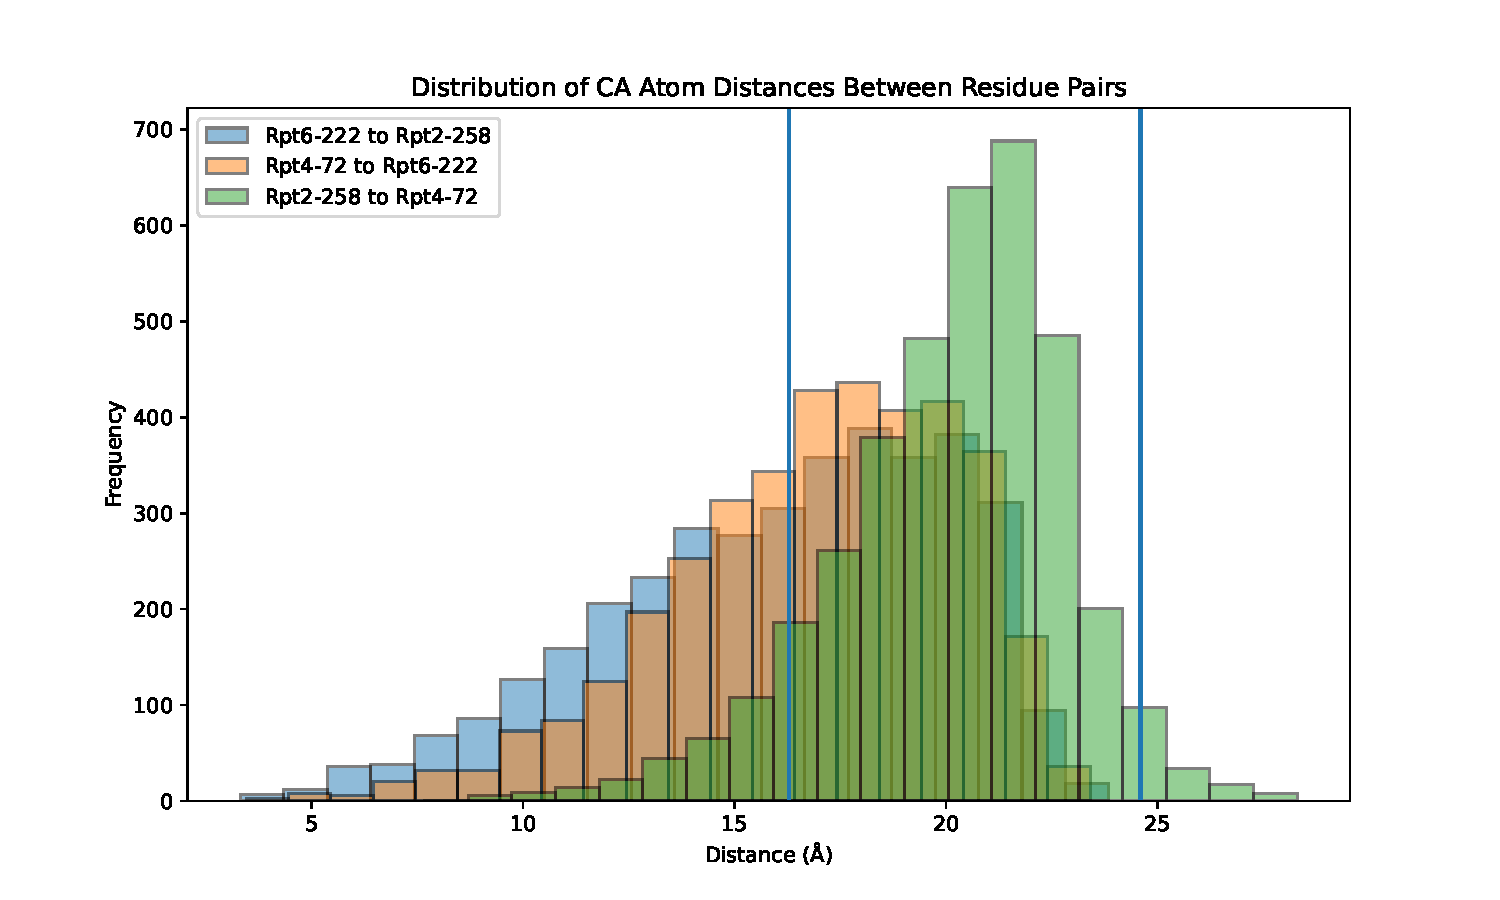
\includegraphics[width=0.41\textwidth]{test-figures/only-bi.pdf}
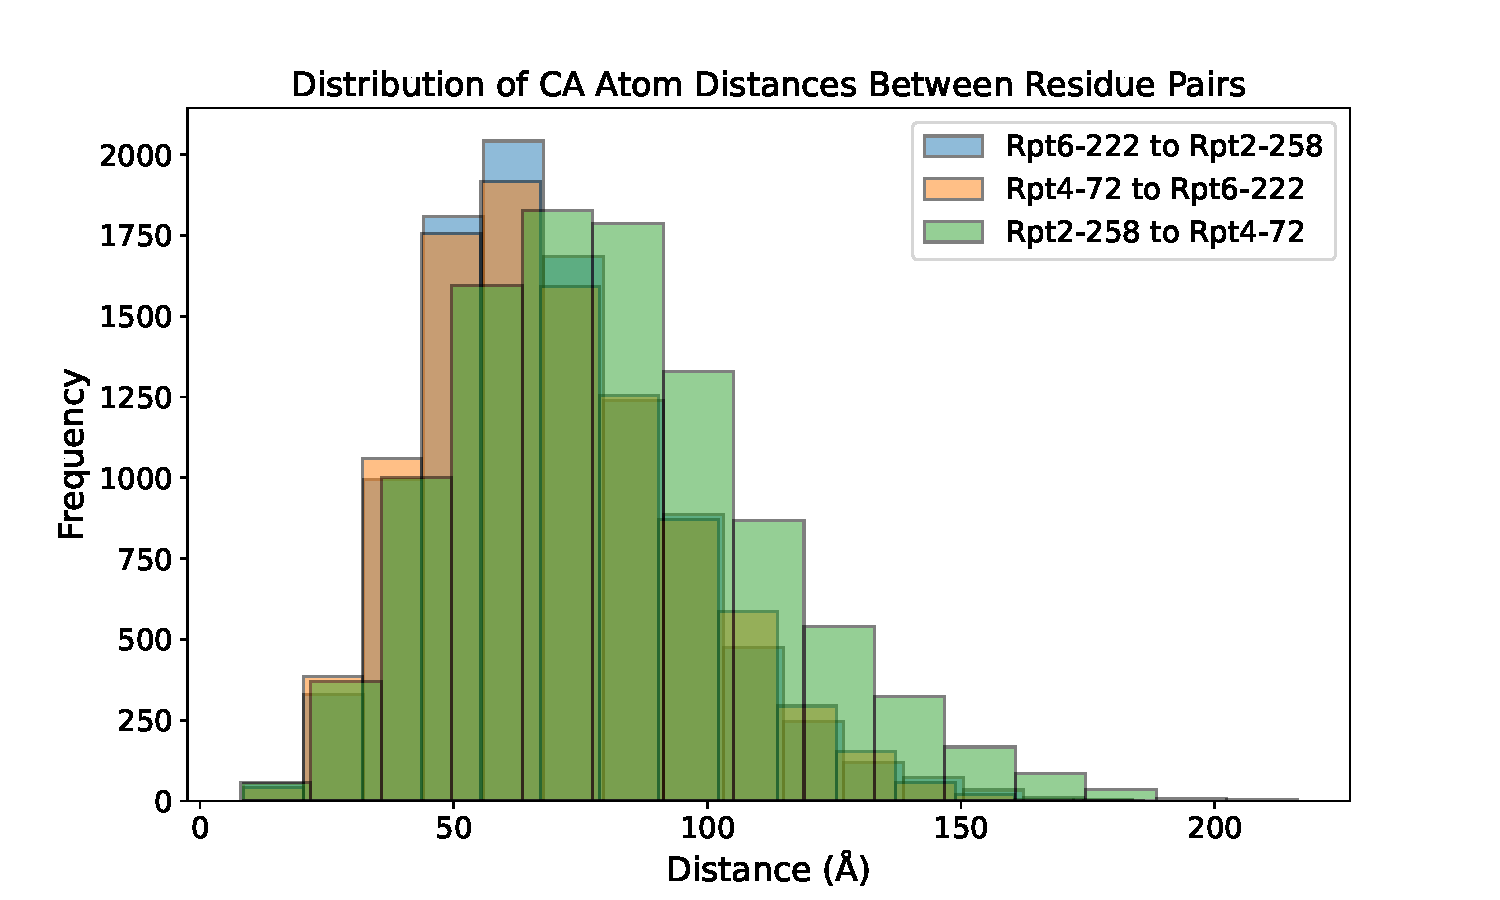
\includegraphics[width=0.41\textwidth]{test-figures/only-tri.pdf}
\caption{On the left, the distance distributions using bifunctional crosslinks and 
on the right, the distance distributions using trifunctional crosslinks (11 {\AA} linker length)}
\end{figure}
%
\begin{minipage}{0.48\textwidth}
  \centering
  \begin{tabular}{lcc}
  \hline
  Residue Pair & Mean (Å) & Std Dev (Å) \\
  \hline
  Pair 1 & 16.1 & 4.0 \\
  Pair 2 & 16.9 & 3.3 \\
  Pair 3 & 20.1 & 2.7 \\
  \hline
  \end{tabular}
  \captionof{table}{Bifunctional crosslinks}
  \end{minipage}
  \hfill
  \begin{minipage}{0.48\textwidth}
  \centering
  \begin{tabular}{lcc}
  \hline
  Residue Pair & Mean (Å) & Std Dev (Å) \\
  \hline
  Pair 1 & 69.5 & 24.7 \\
  Pair 2 & 69.3 & 25.2 \\
  Pair 3 & 81.3 & 30.36 \\
  \hline
  \end{tabular}
  \captionof{table}{Trifunctional crosslinks (11 {\AA} linker)}
  \end{minipage}
\end{frame}
%------------------------------------------------------------------------------
\begin{frame}
\frametitle{Optimizing the crosslinker length}
\begin{figure}
\centering
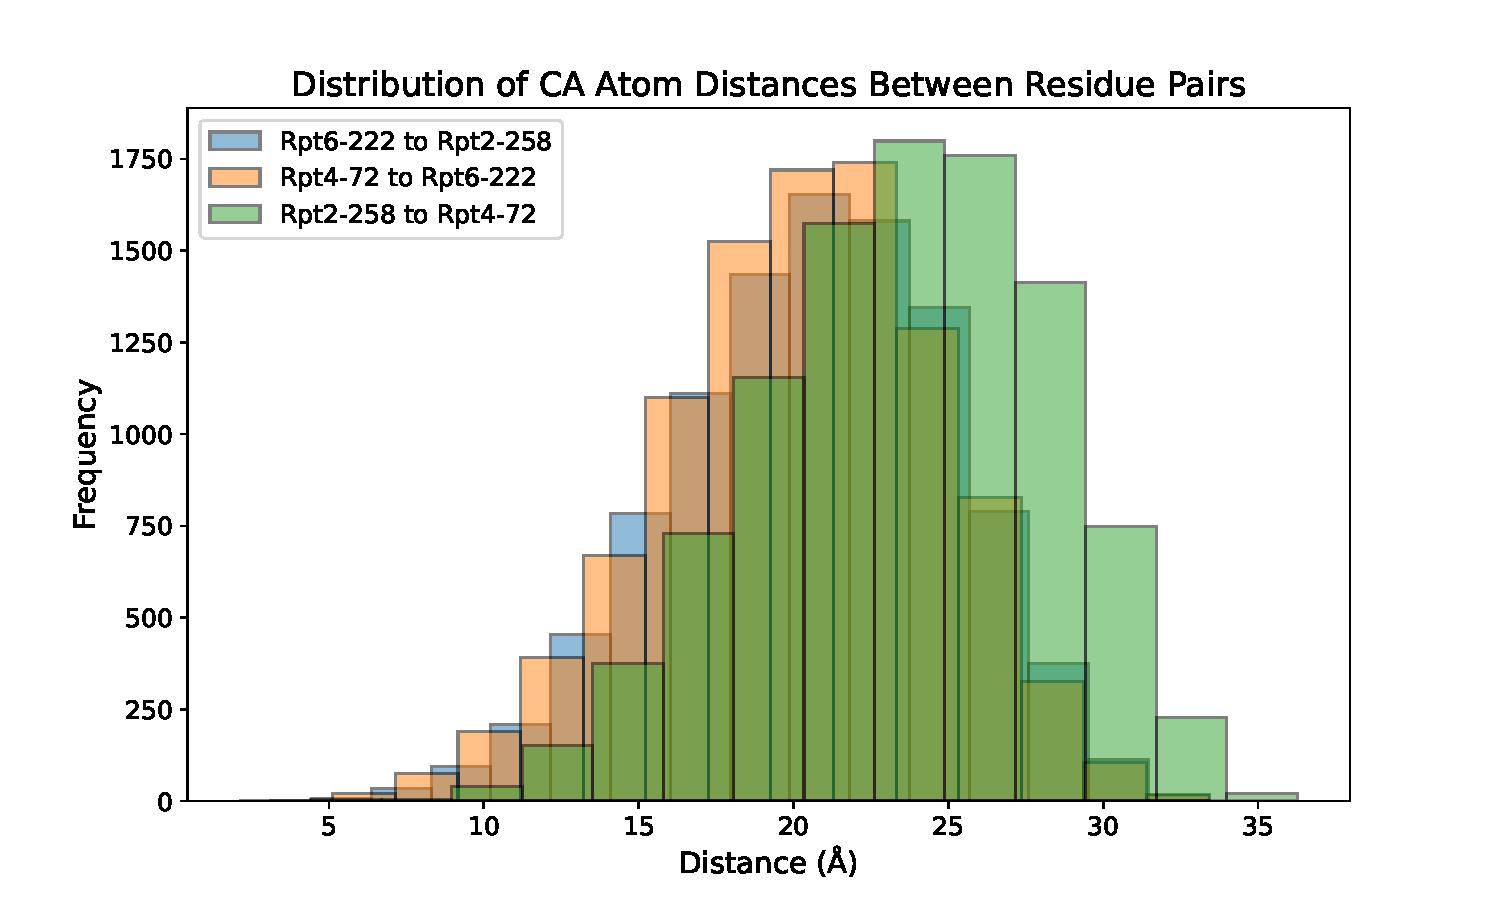
\includegraphics[width=0.41\textwidth]{test-figures/tri-16.pdf}
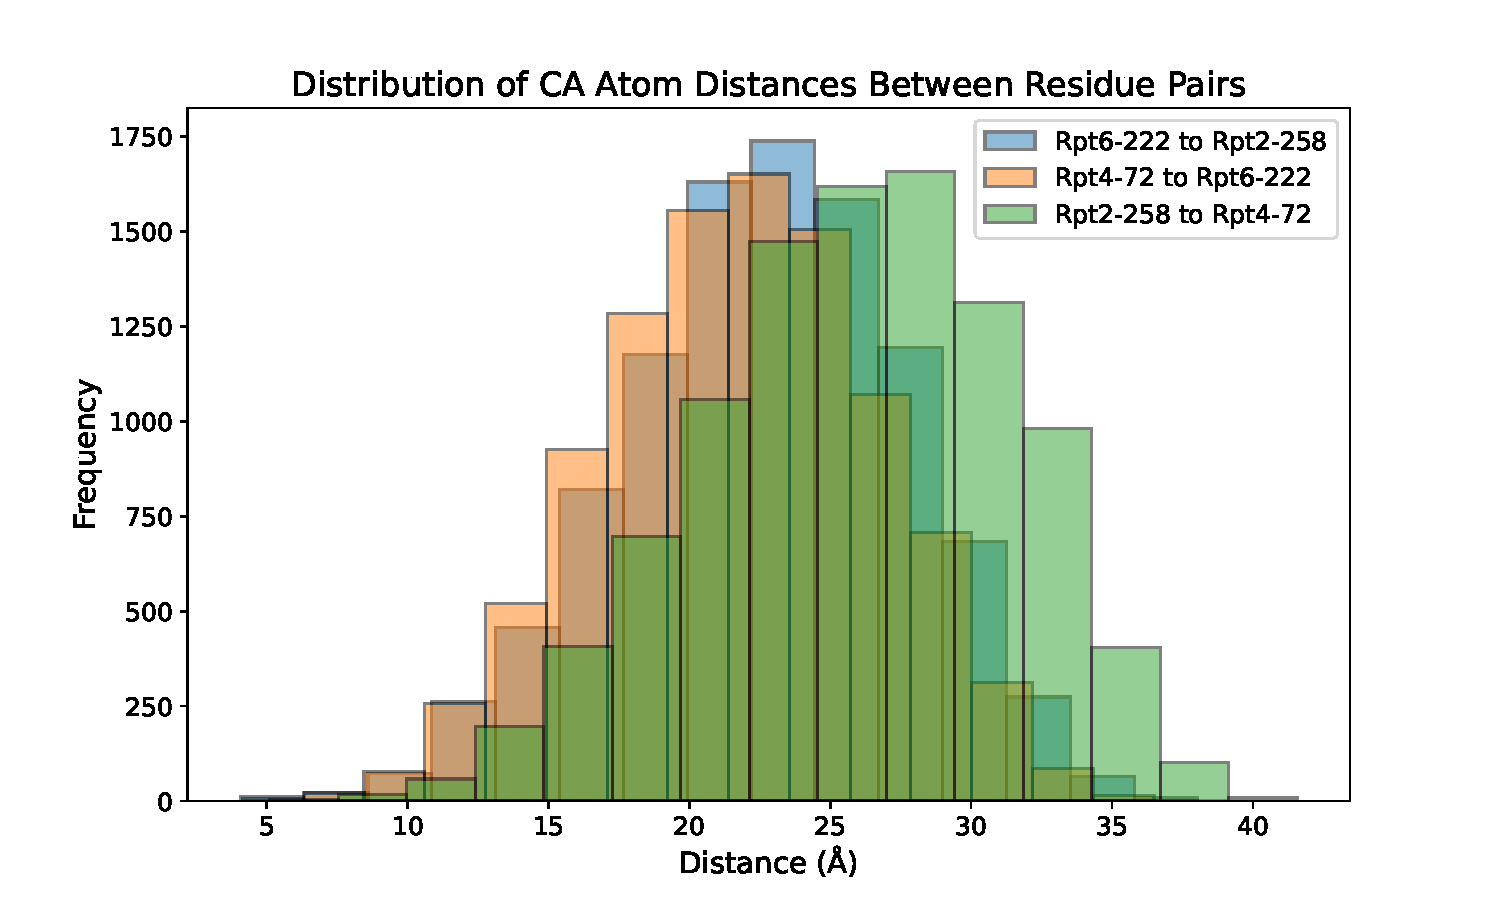
\includegraphics[width=0.41\textwidth]{test-figures/18-tri.pdf}
\caption{On the left, distance distributions using trifunctional crosslinker 
(16 {\AA} linker length) and on the right, the distance distributions 
using trifunctional crosslinks (18 {\AA} linker length)}
\end{figure}
%
\begin{minipage}{0.48\textwidth}
  \centering
  \begin{tabular}{lcc}
  \hline
  Residue Pair & Mean (Å) & Std Dev (Å) \\
  \hline
  Pair 1 & 21.3 & 7.0 \\
  Pair 2 & 20.9 & 8.4 \\
  Pair 3 & 24.7 & 12.3 \\
  \hline
  \end{tabular}
  \captionof{table}{Trifunctional crosslinks (16 {\AA} linker)}
  \end{minipage}
  \hfill
  \begin{minipage}{0.48\textwidth}
  \centering
  \begin{tabular}{lcc}
  \hline
  Residue Pair & Mean (Å) & Std Dev (Å) \\
  \hline
  Pair 1 & 22.7 & 5.0 \\
  Pair 2 & 21.7 & 4.9 \\
  Pair 3 & 25.9 & 5.5 \\
  \hline
  \end{tabular}
  \captionof{table}{Trifunctional crosslinks (18 {\AA} linker)}
  \end{minipage}

%\begin{tabular}
%  {lcc}
%  \hline
%  Residue Pair & Mean (Å) & Std Dev (Å) \\
%  \hline
%  Pair 1 & 25.7 & 6.0 \\
%  Pair 2 & 24.9 & 5.8\\
%  Pair 3 & 28.9 & 6.6 \\
%  \hline
%\end{tabular}
\end{frame}
%------------------------------------------------------------------------------
\begin{frame}
\frametitle{Results for optimized crosslinker length}
\begin{table}
  \centering
  \caption{Comparison of the double and triple XL datasets}
  \begin{tabular}{|c|c|c|c|}
      \hline
                                   & Samp. precision ({\AA}) & Clust. precision & Accuracy\\ \hline
      bifunctional ($n(bi) = 164$) & 4.42  & 3.3 & 14.43 \\\hline
      n($bi \cup tri) = 186$       & 10.68 & 7.3 &  16.09 \\\hline
      XL length = 16 {\AA} with overlap & 8.5   & 5.2 & 15.01 \\\hline
  \end{tabular}
\end{table}
\begin{block}{}
  Simulations with synthetic crosslinks with the optimized crosslinker length
\end{block}
\end{frame}
%------------------------------------------------------------------------------
\begin{frame}
  \frametitle{Modeling with TSTO crosslinker}
  \begin{minipage}{0.48\textwidth}
    \centering
    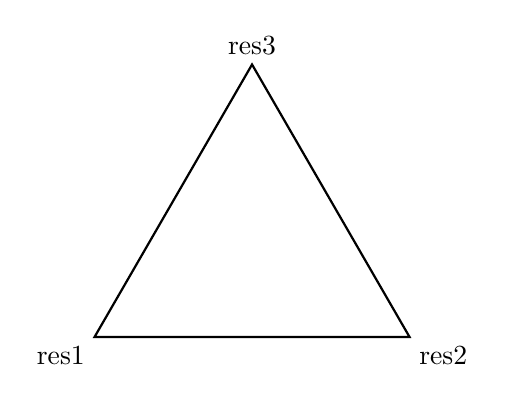
\begin{tikzpicture}
      % Define the coordinates of the triangle corners
      \coordinate (A) at (0, 0);
      \coordinate (B) at (4, 0);
      \coordinate (C) at (2, 3.46); % Height of an equilateral triangle with side length 4

      % Draw the triangle
      \draw[thick] (A) -- (B) -- (C) -- cycle;

      % Label the corners
      \node[below left] at (A) {res1};
      \node[below right] at (B) {res2};
      \node[above] at (C) {res3};
    \end{tikzpicture}
    \vspace{0.5cm}
    \centering
    Modeling with triangular geometrical restraints
  \end{minipage}
  \hfill
  \begin{minipage}{0.48\textwidth}
    \centering
    \begin{tikzpicture}
      % Define the coordinates of the triangle corners
      \coordinate (A) at (0, 0);
      \coordinate (B) at (4, 0);
      \coordinate (C) at (2, 3.46); % Height of an equilateral triangle with side length 4

      % Calculate the center of the triangle
      \coordinate (D) at (2, 1.15); % Centroid of the equilateral triangle

      % Draw lines from the dummy bead to the corners
      \draw[thick] (D) -- (A);
      \draw[thick] (D) -- (B);
      \draw[thick] (D) -- (C);

      % Draw the dummy bead
      \filldraw[black] (D) circle (2pt);
      \node[above right] at (D) {dummy bead};

      % Label the corners
      \node[below left] at (A) {res1};
      \node[below right] at (B) {res2};
      \node[above] at (C) {res3};
    \end{tikzpicture}
    \vspace{0.5cm}
    \centering
    Modeling with a dummy bead
  \end{minipage}
\end{frame}
%
\begin{frame}
\frametitle{tri-XL connected residues linked via dummy bead}
\begin{tikzpicture}
  % Define the coordinates of the triangle corners
  \coordinate (A) at (0, 0);
  \coordinate (B) at (4, 0);
  \coordinate (C) at (2, 3.46); % Height of an equilateral triangle with side length 4

  % Calculate the center of the triangle
  \coordinate (D) at (2, 1.15); % Centroid of the equilateral triangle

  % Draw lines from the dummy bead to the corners
  \draw[thick] (D) -- (A);
  \draw[thick] (D) -- (B);
  \draw[thick] (D) -- (C);

  % Draw the dummy bead
  \filldraw[black] (D) circle (2pt);
  \node[above right] at (D) {dummy bead};

  % Label the corners
  \node[below left] at (A) {res1};
  \node[below right] at (B) {res2};
  \node[above] at (C) {res3};
\end{tikzpicture}
%
\begin{table}
  \centering
  \caption{Comparison of the bi- and trifunctional XL datasets}
  \begin{tabular}{|c|c|c|c|}
      \hline
                                   & Samp. precision ({\AA}) & Clust. precision & Accuracy\\ \hline
      bifunctional ($n(bi) = 164$) & 4.42  & 3.3 & 14.43 \\\hline
      n($bi \cup tri) = 186$       & 10.68 & 7.3 &  16.09 \\\hline
      XL length = 16 {\AA} with overlap & 8.5   & 5.2 & 15.01 \\\hline
  \end{tabular}
\end{table}
\end{frame}
%
\begin{frame}
\frametitle{tri-XL connected residues linked via regular XL restraints}
%\begin{itemize}
%  \item No dummy bead used
%  \item Regular XL restraints used to connect the residues with lengths of 21 and 18 {\AA} for the simulations.
%  \item Simulations run with inclusion of overlap removed bi-functional data
%\end{itemize}
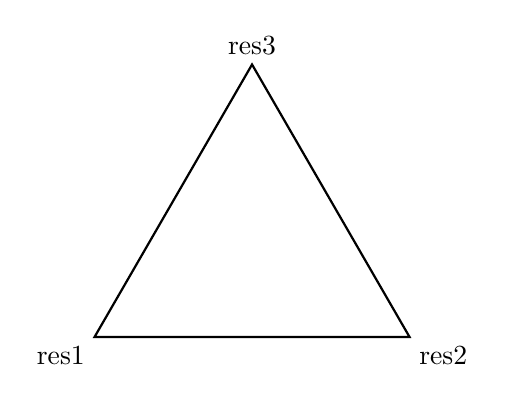
\begin{tikzpicture}
  % Define the coordinates of the triangle corners
  \coordinate (A) at (0, 0);
  \coordinate (B) at (4, 0);
  \coordinate (C) at (2, 3.46); % Height of an equilateral triangle with side length 4

  % Draw the triangle
  \draw[thick] (A) -- (B) -- (C) -- cycle;

  % Label the corners
  \node[below left] at (A) {res1};
  \node[below right] at (B) {res2};
  \node[above] at (C) {res3};
\end{tikzpicture}

\begin{table}
  \centering
  \caption{Results for the tri-XL connected residues linked via regular XL restraints}
  \begin{tabular}{|c|c|c|c|c|}
      \hline
                                   & Samp. precision ({\AA}) & Cl. pop. & Cl. precision ({\AA}) & Accuracy ({\AA})\\ \hline
      186 XLs, XL $=$ 24 {\AA} & 4.408  & 23600 & 3.41 & 14.90\\ \hline
      186 XLs, XL $=$ 21 {\AA} & 4.377  & 24000 & 3.36 & 14.57\\ \hline
      186 XLs, XL $=$ 18 {\AA} & 4.38   & 16000 & 3.32 & 13.51\\ \hline
  \end{tabular}
\end{table}
\begin{table}
  \centering
  \caption{Comparison to modeling done with only bifunctional XLs}
  \begin{tabular}{|c|c|c|c|}
      \hline
                                   & Samp. precision ({\AA}) & Cl. precision & Accuracy\\ \hline
      bifunctional ($n(bi) = 164$) & 4.42  & 3.3 & 14.43 \\\hline
  \end{tabular}
\end{table}

\end{frame}
%
\begin{frame}[fragile=singleslide]
\frametitle{upper bound distance restraint}
\begin{verbatim}
  disres = IMP.pmi.restraints.basic.DistanceRestraint(root_hier, 
  tuple1, tuple2, min = 0.0, max=16.0, resolution=1.0, kappa=1.0)
  \end{verbatim}
  \begin{figure}
    \centering
    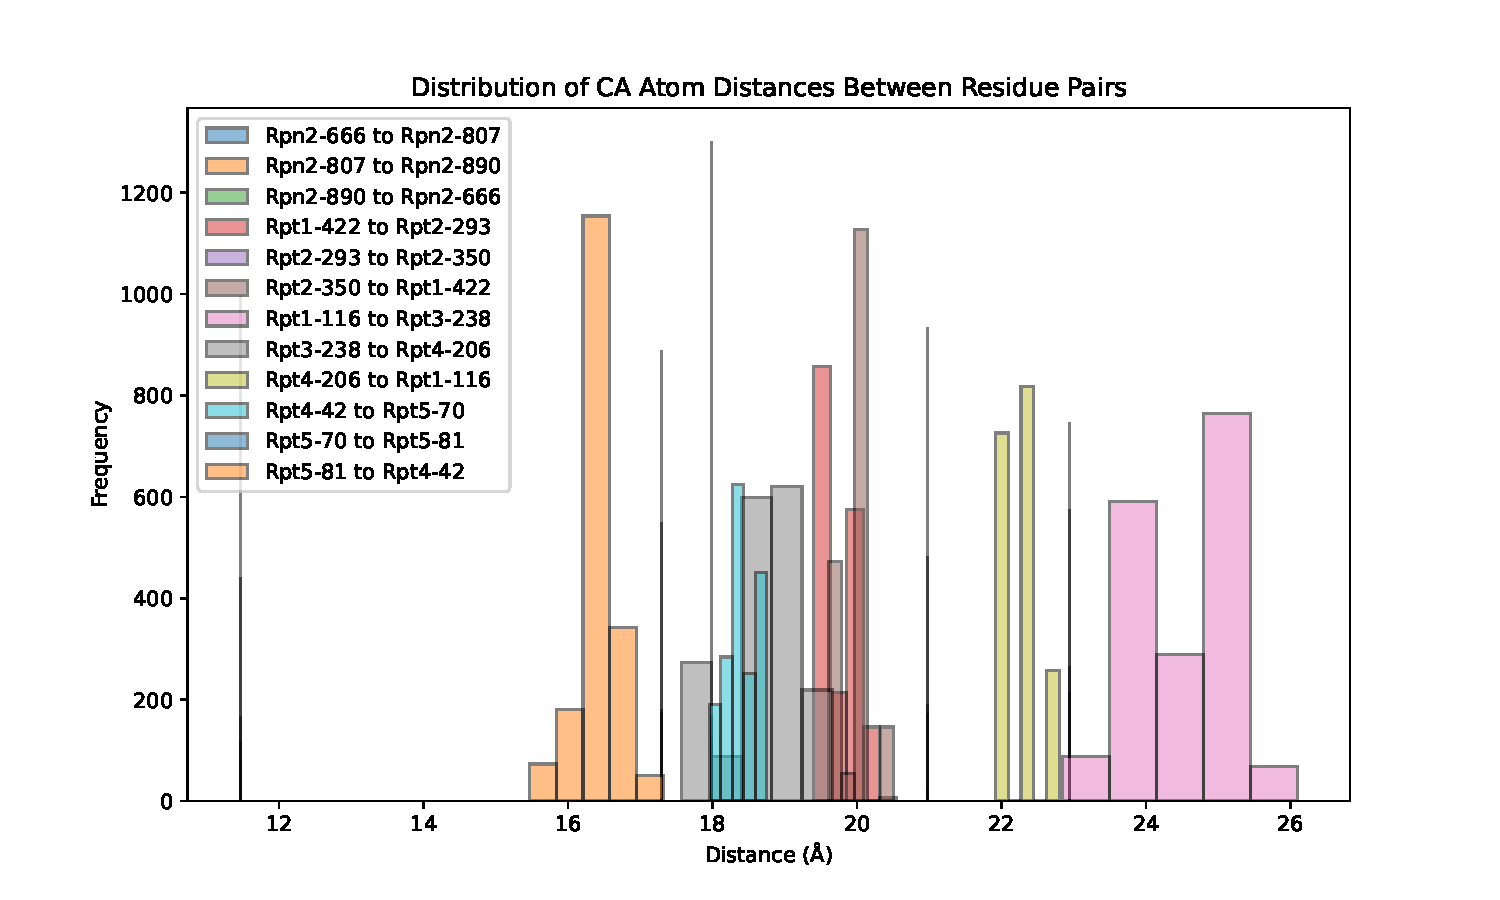
\includegraphics[scale=0.2]{test-figures/disres_dist.pdf}
    \caption{Distribution of distances when upper bound distance restraint is 
    applied to the residues that are linked by trifunctional Xl for a 2000 step MCMC trajectory.}
  \end{figure}
  \begin{table}
    \centering
    \caption{Results for the tri-XL connected residues linked via distance restraints}
    \begin{tabular}{|c|c|c|c|c|}
        \hline
                                     & Samp. precision ({\AA}) & Cl. pop. & Cl. precision ({\AA}) & Accuracy ({\AA})\\ \hline
        186 XLs & 2.26  & 29000 & 1.58 & 15.06\\ \hline
        %186 XLs, XL $=$ 21 {\AA} & 4.377  & 24000 & 3.36 & 14.57\\ \hline
        %186 XLs, XL $=$ 18 {\AA} & 4.38   & 16000 & 3.32 & 13.51\\ \hline
    \end{tabular}
  \end{table}
\end{frame}
%
\begin{frame}
\frametitle{Comparison with DSSO crosslinking data}
  \begin{figure}
   \centering
   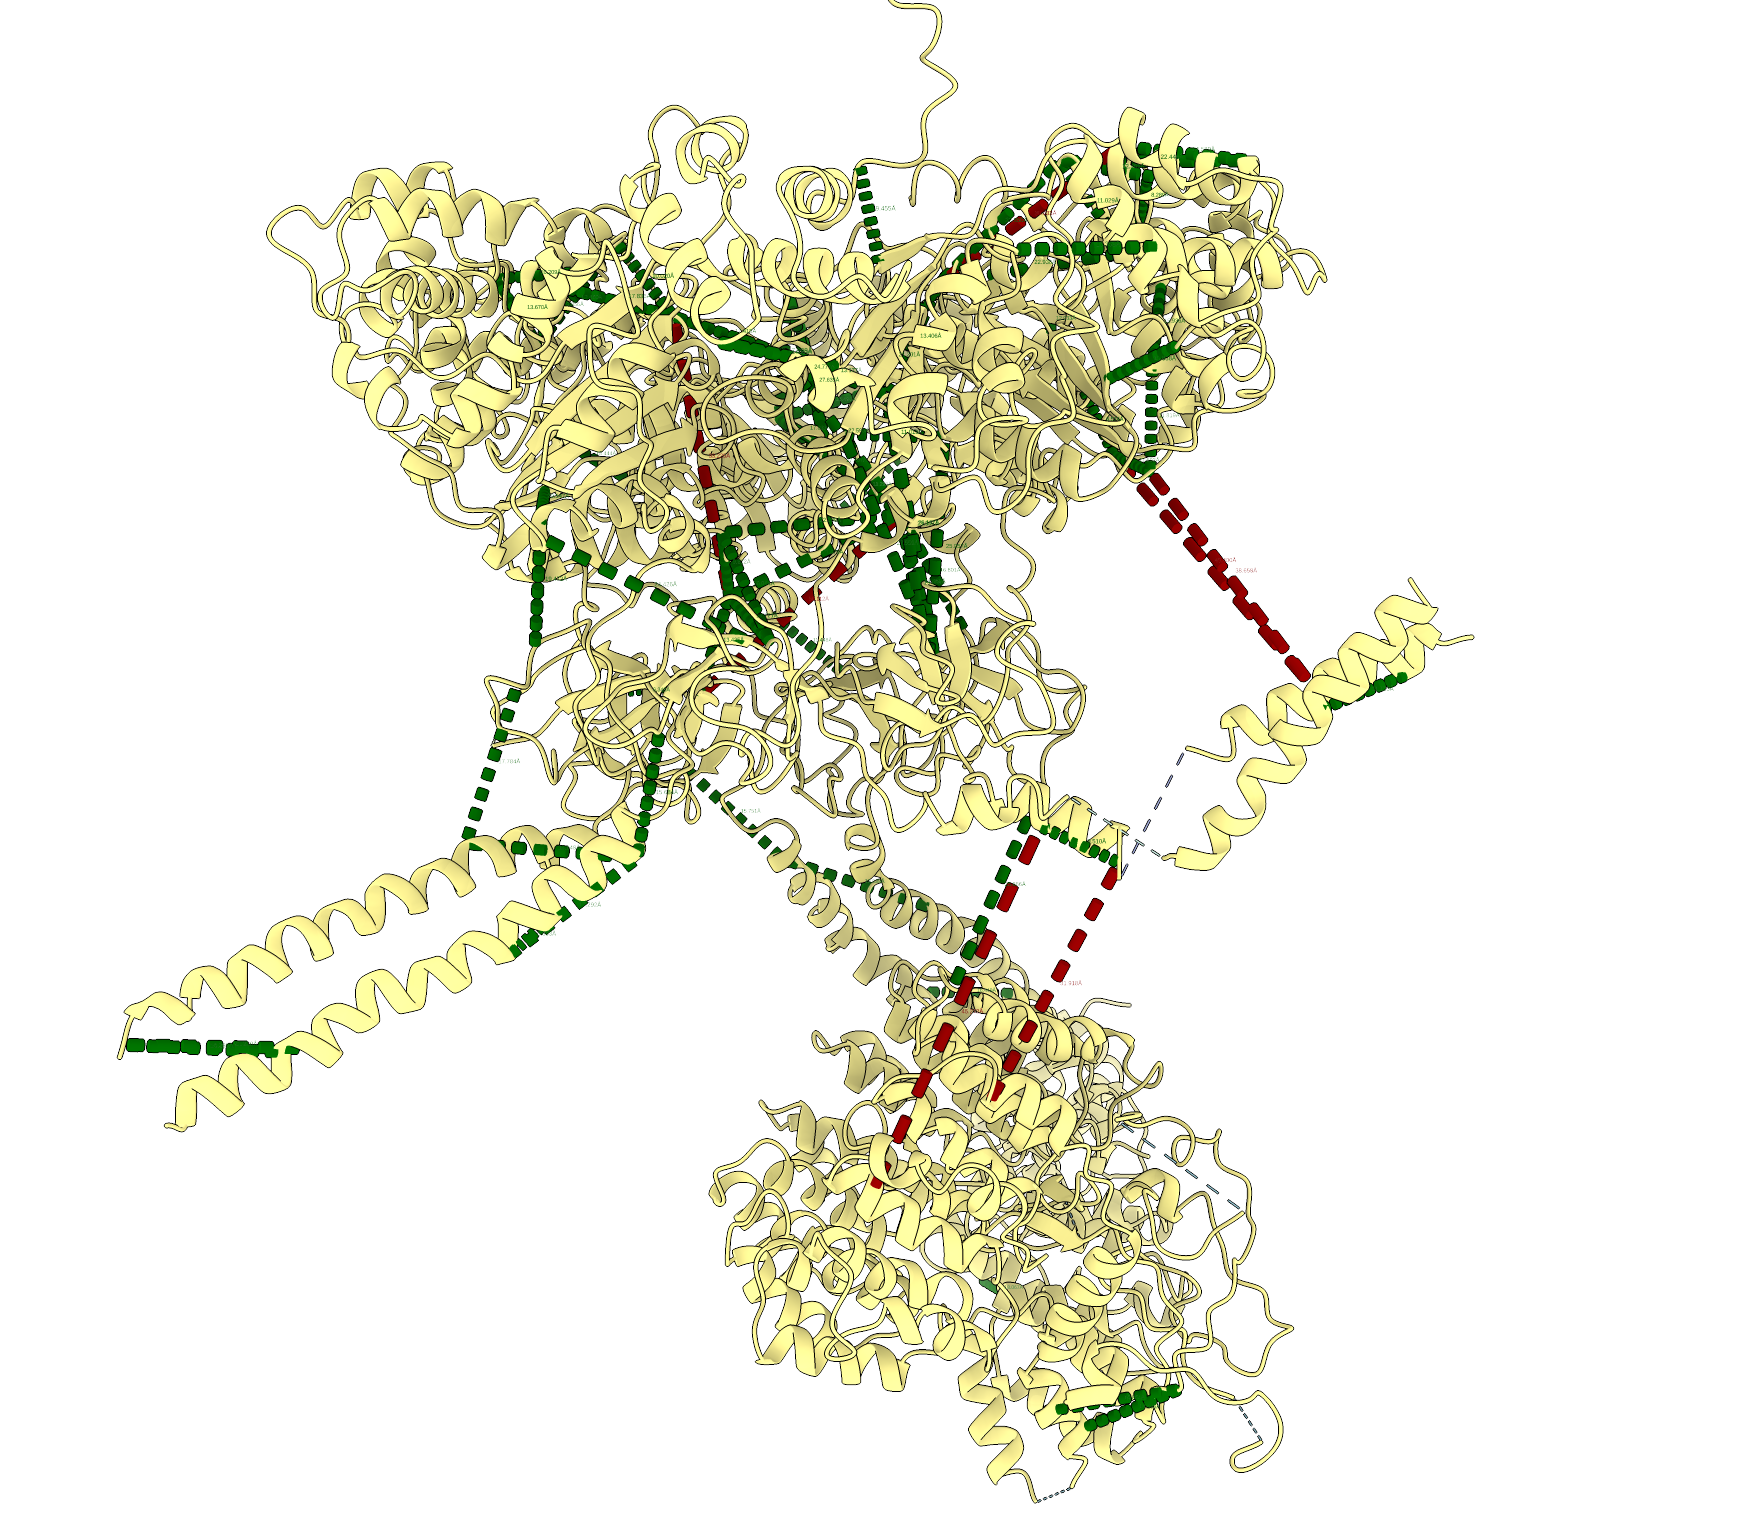
\includegraphics[width=0.4\textwidth]{figures/dsso-mapped-xls.png}
   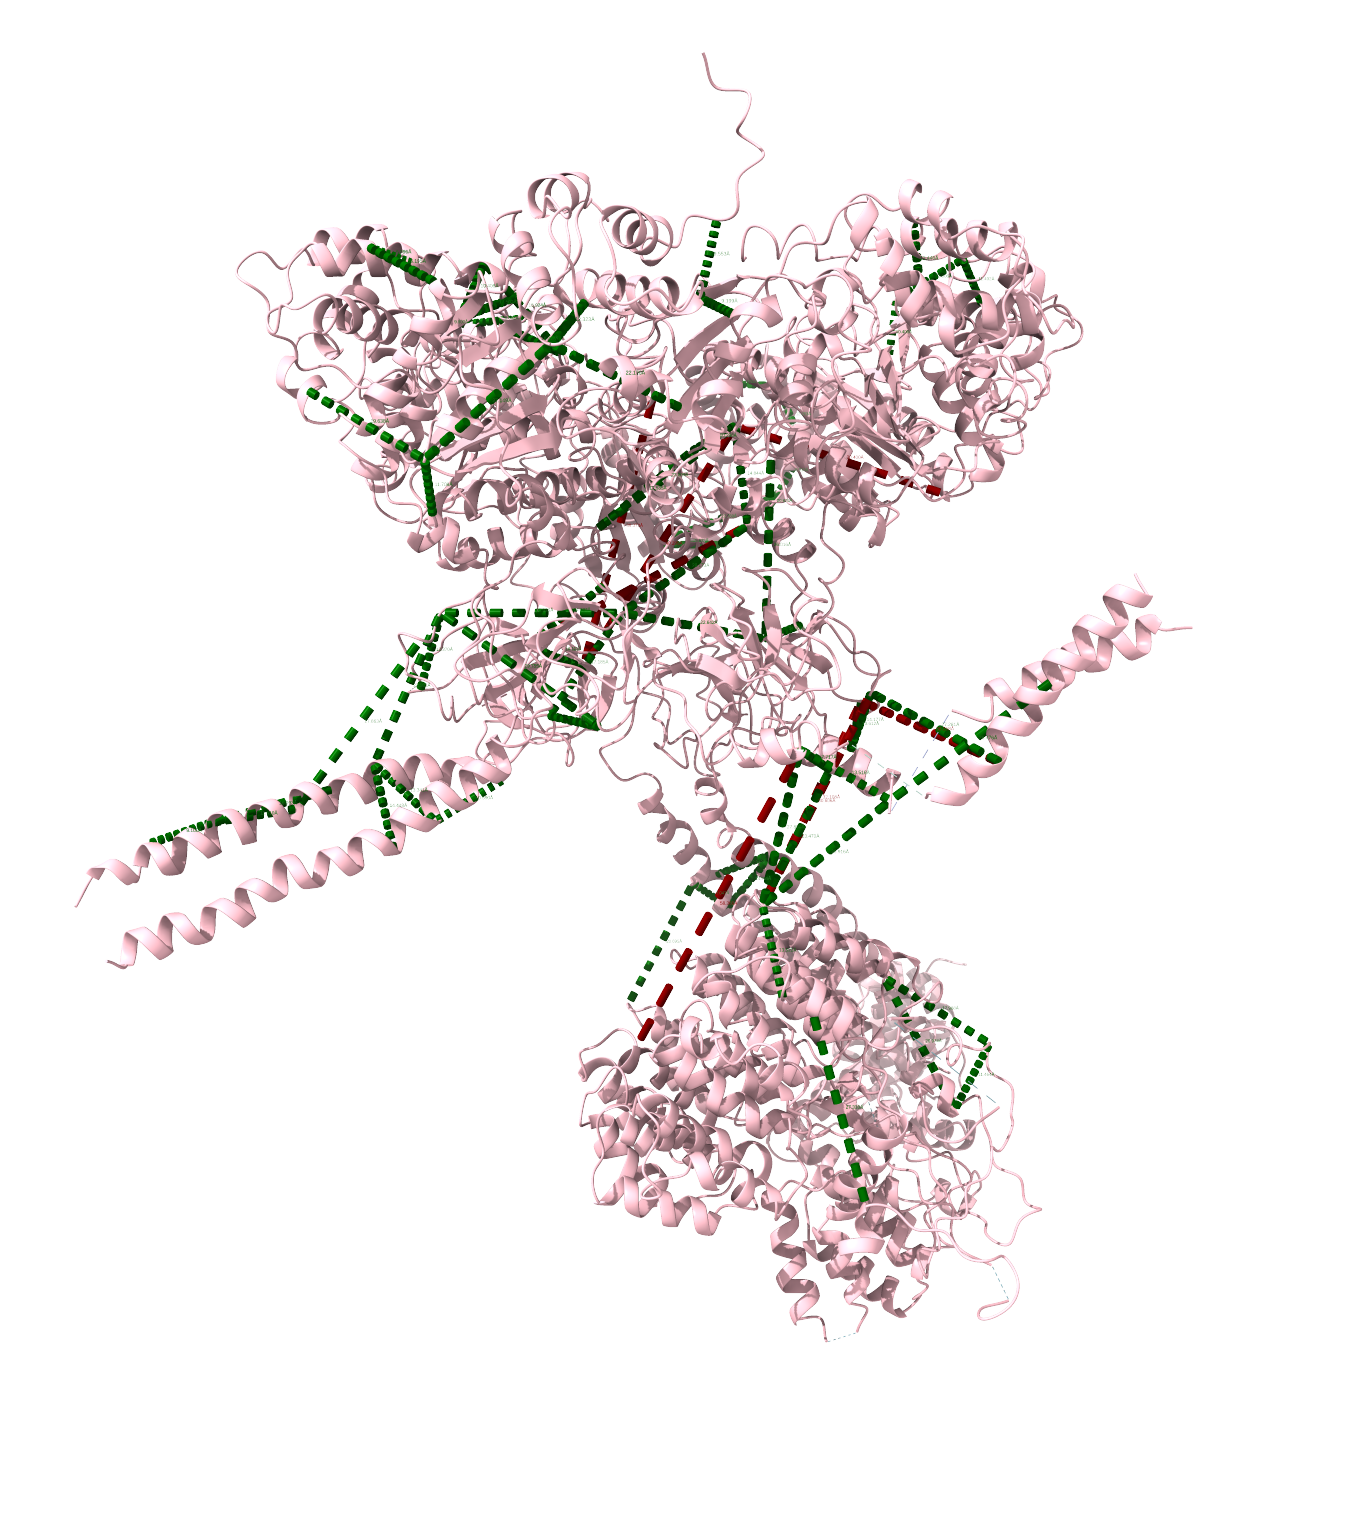
\includegraphics[width=0.4\textwidth]{test-figures/unique_to_tsto.png}
   \caption{XLs identified using DSSO XL (left) and Xls that are unique to TSTO (right) mapped onto the base subcomplex structure}
   There are $\sim 100$ more unique crosslinks identified using TSTO.
  \end{figure}
\end{frame}
%
\begin{frame}
  \frametitle{Distance distribution of experimental trifunctional XLs}
  \centering
  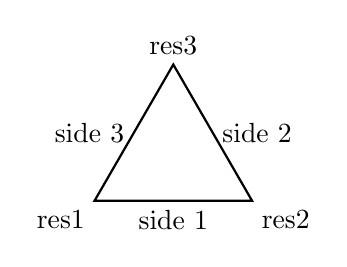
\begin{tikzpicture}[scale=0.5]
    % Define the coordinates of the triangle corners
    \coordinate (A) at (0, 0);
    \coordinate (B) at (4, 0);
    \coordinate (C) at (2, 3.46); % Height of an equilateral triangle with side length 4
  
    % Draw the triangle
    \draw[thick] (A) -- (B) -- (C) -- cycle;
  
    % Label the corners
    \node[below left] at (A) {res1};
    \node[below right] at (B) {res2};
    \node[above] at (C) {res3};
  
    % Label the sides
    \node[below] at ($(A)!0.5!(B)$) {side 1};
    \node[right] at ($(B)!0.5!(C)$) {side 2};
    \node[left] at ($(C)!0.5!(A)$) {side 3};
  \end{tikzpicture}
  %
  \begin{table}
    \centering
    \caption{Distance distribution of experimental trifunctional XLs}
  \begin{tabular}{lrrrrr}
    \toprule
    Side & Mean ({\AA}) & Std ({\AA}) & Max ({\AA}) & Min ({\AA}) & Count $> 30${\AA} \\
    \midrule
    side 1 & 13.27 & 3.53 & 24.73 & 6.80 & 0 \\
    side 2 & 25.16 & 16.54 & 77.91 & 10.59 & 8 \\
    side 3 & 30.93 & 19.79 & 95.91 & 14.44 & 11 \\
    \bottomrule
    \end{tabular}   
  \end{table} 
  \begin{block}
    {}
    \begin{itemize}
      \item There are 35 experimental trifunctional crosslinks identified for the proteasome
      \item The distances are obtained by mapping the XLs onto the pdb structure with code: 5GJR
    \end{itemize}
    \end{block}
\end{frame}
%
\begin{frame}
\frametitle{Working with synthetic XL data}
%
\begin{figure}
  \centering
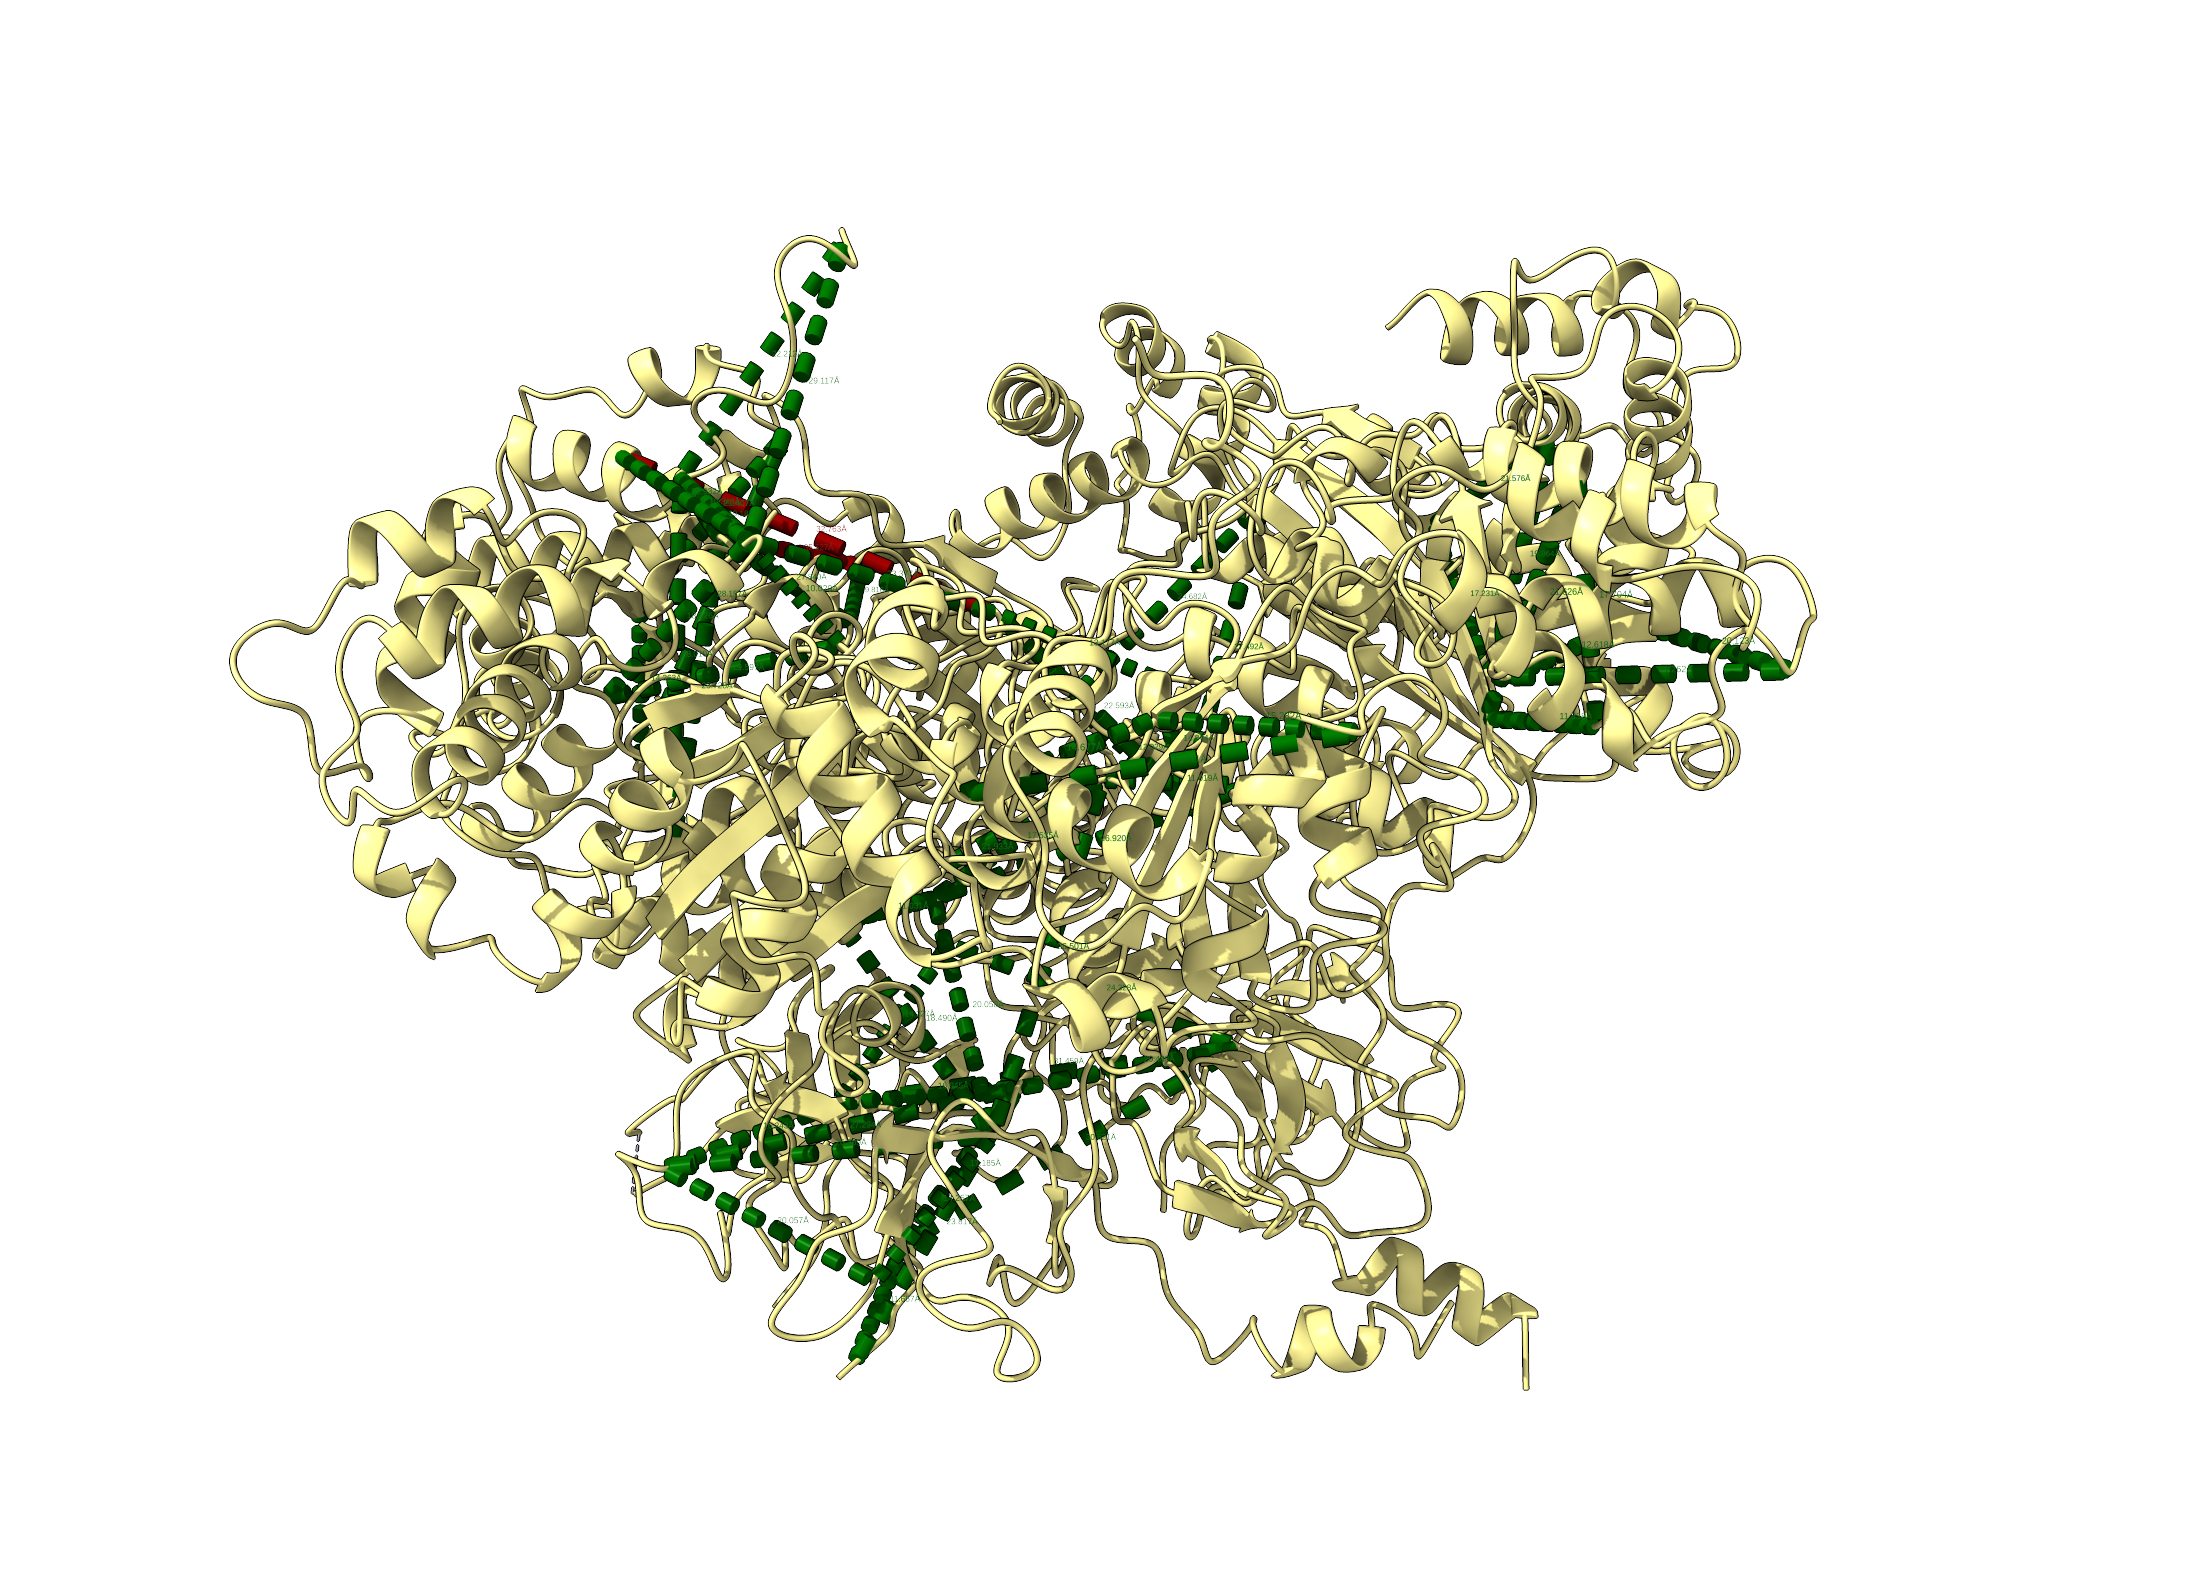
\includegraphics[width=0.3\textwidth]{test-figures/20_syn.png}
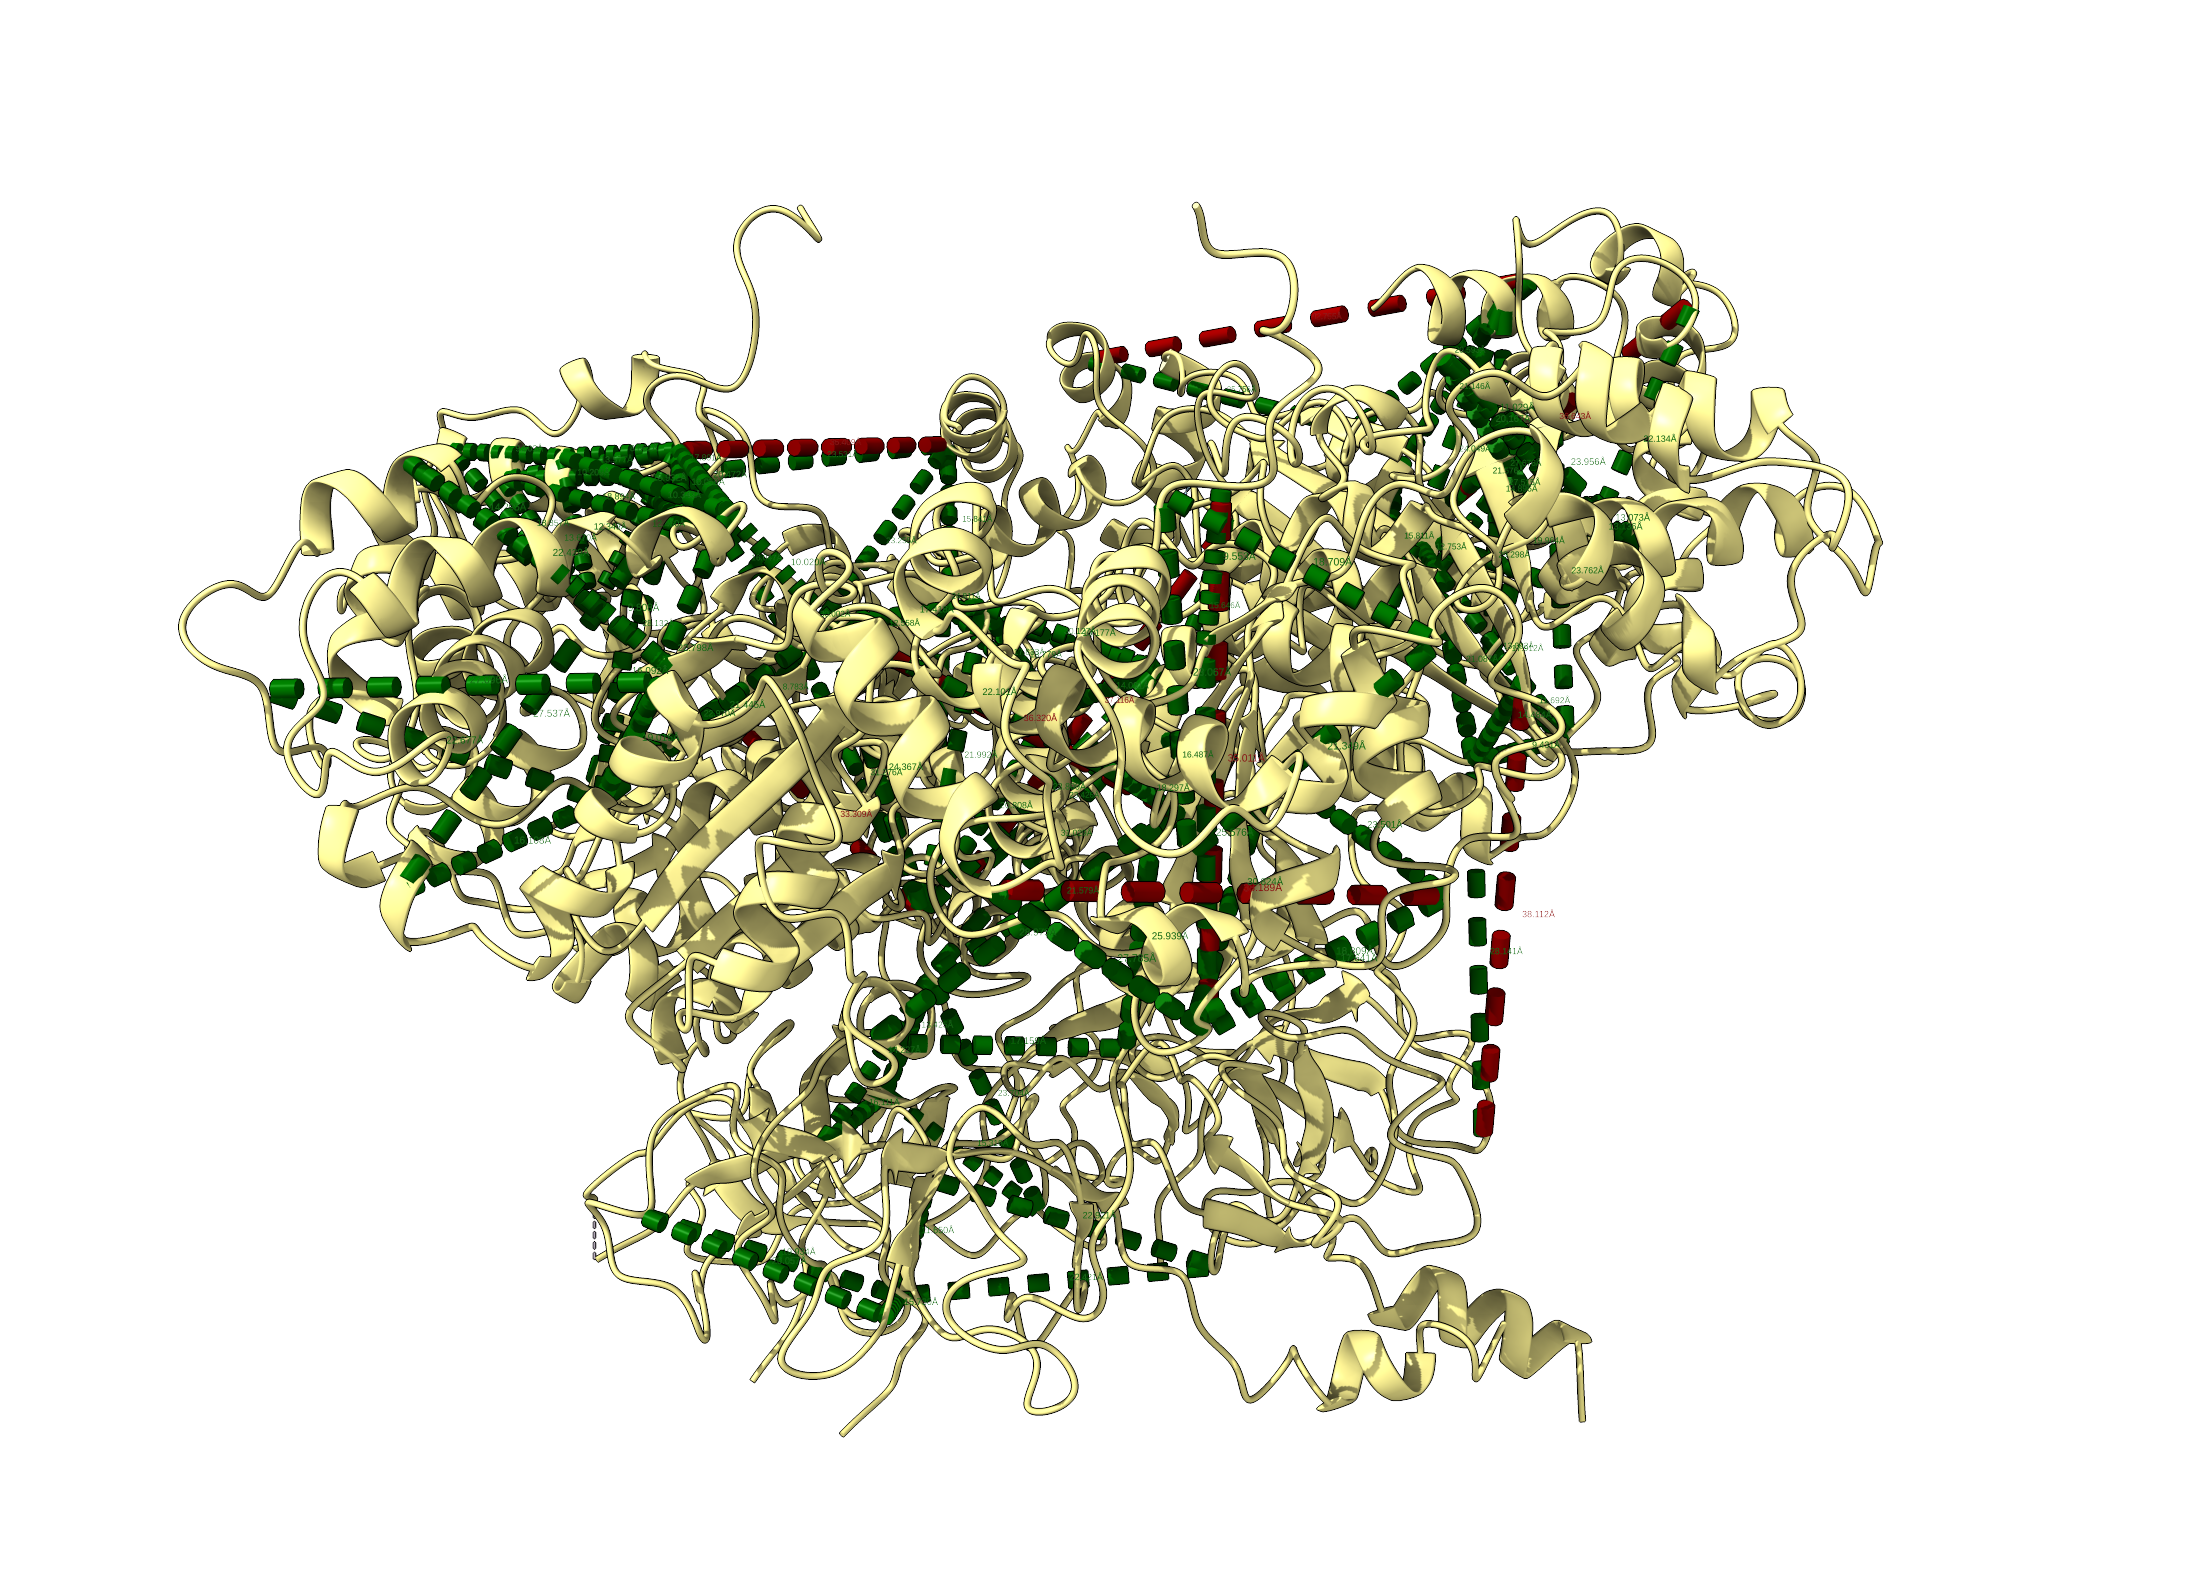
\includegraphics[width=0.3\textwidth]{test-figures/40_syn.png}
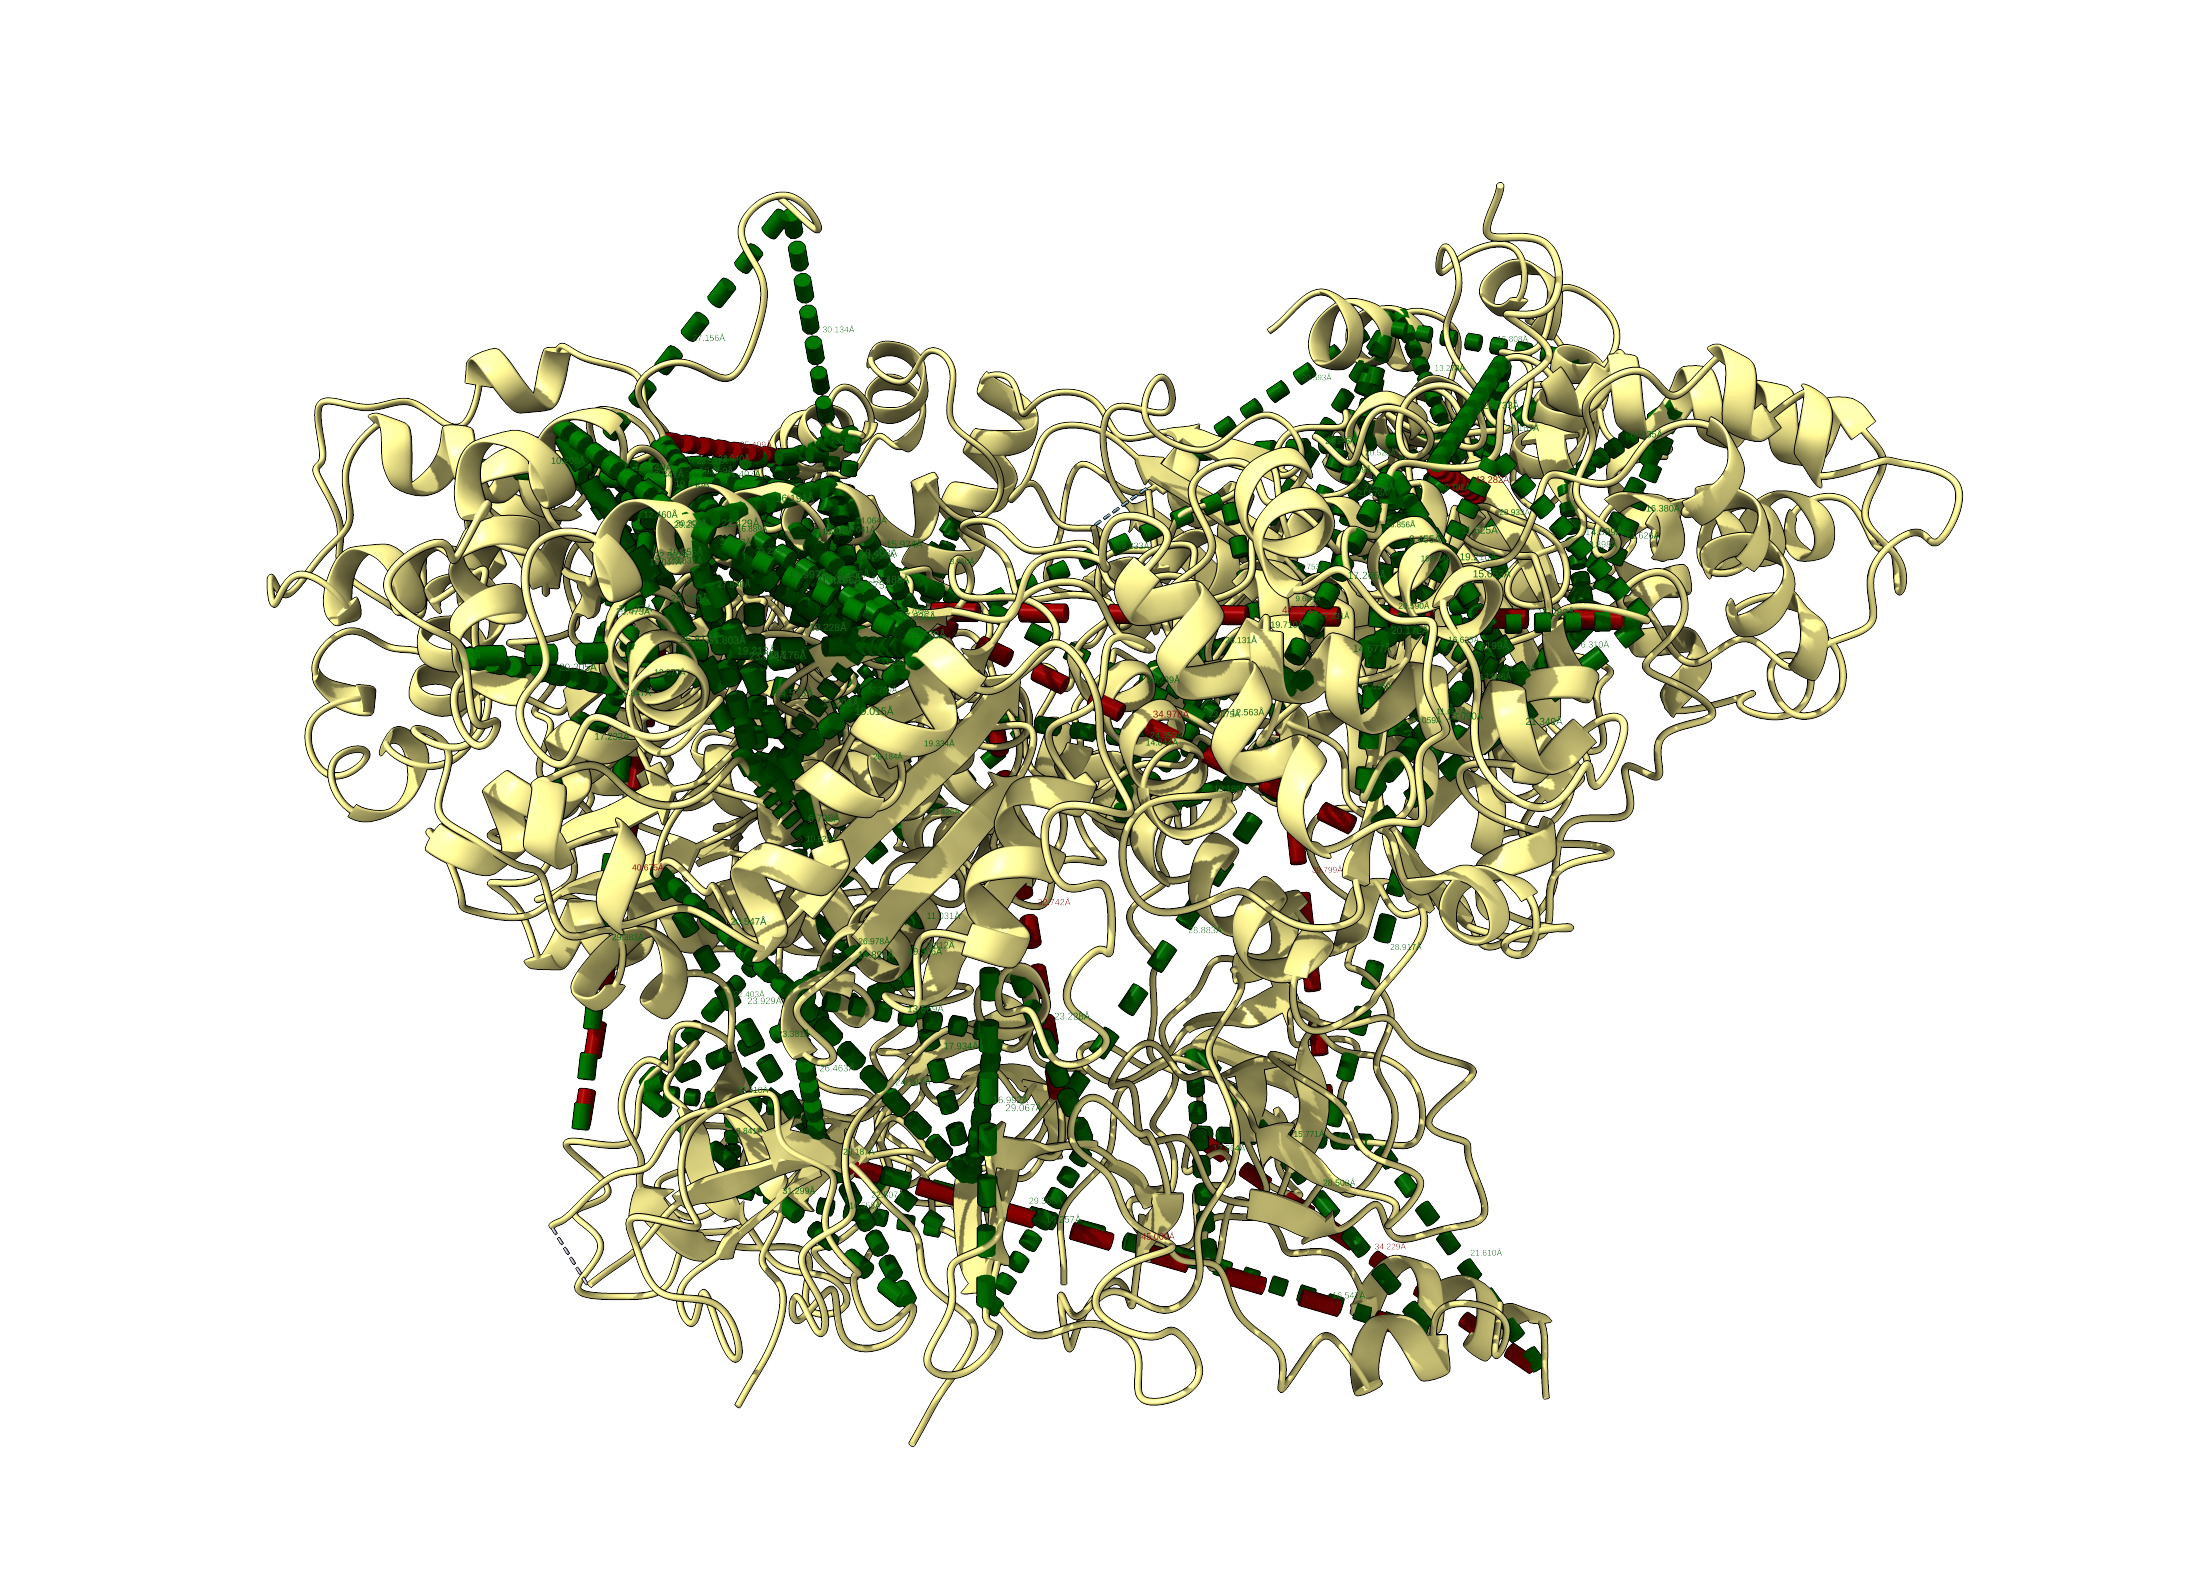
\includegraphics[width=0.3\textwidth]{test-figures/60_syn.png}
\caption{20, 40 and 60 synthetic crosslinks mapped onto the base subcomplex}
\end{figure}
\end{frame}
%------------------------------------------------------------------------------
\begin{frame}
\frametitle{Synthetic data}
\begin{table}[htbp]
  \centering
  \caption{20 trifunctional and 20 bifunctional crosslinks}
  \begin{tabular}{|c|ccc|ccc|ccc|}
      \hline
      & \multicolumn{3}{c|}{Sam. pr. ({\AA})} 
      & \multicolumn{3}{c|}{Cl. pop.} 
      & \multicolumn{3}{c|}{Cl. pr.} \\ \hline
      & rep1 & rep2 & rep3 
      & rep1 & rep2 & rep3 
      & rep1 & rep2 & rep3 \\ \hline
      star 
        & 10.7 & 4.8 & 20.5 
        & 1938  & 1912 & 9941
        & 8.7 & 4.0 & 14.9\\ \hline
      triangle 
        & 4.0 & 4.0 & 8.0 
        & 2199 & 7063 & 9032 
        &  3.2 & 2.1 & 5.1 \\ \hline
      bi 
        & 4.0 & 24.0 & 4.0  
        & 2791 & 9904 & 9734 
        & 3.1 & 14.3 & 2.8  \\ \hline
  \end{tabular}
\end{table}
%
\begin{table}[htbp]
  \centering
  \caption{20 trifunctional and 20 bifunctional crosslinks}
  \begin{tabular}{|c|ccc|}
      \hline 
      & \multicolumn{3}{c|}{Acc.} \\ \hline
      & rep1 & rep2 & rep3 \\ \hline
      star 
        &  34.8 & 19.7 & 18.9 \\ \hline
      triangle 
        & 35.5 & 18.2 & 15.3 \\ \hline
      bi 
        & 36.2 & 33.1 & 18.5 \\ \hline
  \end{tabular}
\end{table}
\end{frame}


\begin{frame}
  \frametitle{Synthetic data}
  \begin{table}[htbp]
    \centering
    \caption{40 trifunctional and 40 bifunctional crosslinks}
    \begin{tabular}{|c|ccc|ccc|ccc|}
        \hline
        & \multicolumn{3}{c|}{Sam. pr. ({\AA})} 
        & \multicolumn{3}{c|}{Cl. pop.} 
        & \multicolumn{3}{c|}{Cl. pr.} \\ \hline
        & rep1 & rep2 & rep3 
        & rep1 & rep2 & rep3 
        & rep1 & rep2 & rep3 \\ \hline
        star 
          & 6.8 & 2.9 & 4.9  
          & 7526  & 2135 & 4680
          & 5.7 & 2.6 & 3.8\\ \hline
        triangle 
          &  &  &  
          & 9999 & 9863 & 5901  
          &   &  &  \\ \hline
        bi 
          &  &  &   
          & 9649 & 9951 & 9700 
          &  &  &   \\ \hline
    \end{tabular}
  \end{table}
  %
  \begin{table}[htbp]
    \centering
    \caption{40 trifunctional and 40 bifunctional crosslinks}
    \begin{tabular}{|c|ccc|}
        \hline 
        & \multicolumn{3}{c|}{Acc.} \\ \hline
        & rep1 & rep2 & rep3 \\ \hline
        star 
          &  9.5 & 11.9 & 14.4 \\ \hline
        triangle 
          & 8.5 & 13.7 & 8.6 \\ \hline
        bi 
          & 9.3 & 27.5 & 11.6 \\ \hline
    \end{tabular}
  \end{table}
  \end{frame}


\begin{frame}
  \frametitle{Synthetic data}
  \begin{table}[htbp]
    \centering
    \caption{60 trifunctional and 60 bifunctional crosslinks}
    \begin{tabular}{|c|ccc|ccc|ccc|}
        \hline
        & \multicolumn{3}{c|}{Sam. pr. ({\AA})} 
        & \multicolumn{3}{c|}{Cl. pop.} 
        & \multicolumn{3}{c|}{Cl. pr.} \\ \hline
        & rep1 & rep2 & rep3 
        & rep1 & rep2 & rep3 
        & rep1 & rep2 & rep3 \\ \hline
        star 
          &  &  &  
          & 7500  & 2100 & 4700
          &  &  & \\ \hline
        triangle 
          & 2.0 & 2.0 & 2.0
          & 9900 &  9700 & 5800 
          & 1.1  & 1.3 & 1.4 \\ \hline
        bi 
          & 2.0 & 2.0 & 2.0  
          & 9000 & 10000 & 8300 
          & 1.3 & 1.15 & 1.1  \\ \hline
    \end{tabular}
  \end{table}
  %
  \begin{table}[htbp]
    \centering
    \caption{60 trifunctional and 60 bifunctional crosslinks}
    \begin{tabular}{|c|ccc|}
        \hline 
        & \multicolumn{3}{c|}{Acc.} \\ \hline
        & rep1 & rep2 & rep3 \\ \hline
        star 
          & 8.7  & 10.6 & 10.89 \\ \hline
        triangle 
          & 8.5 & 8.8 & 7.9 \\ \hline
        bi 
          & 8.7 & 9.1 &  10.5\\ \hline
    \end{tabular}
  \end{table}
  \end{frame}
%
\begin{frame}
  \frametitle{Synthetic data statistics}
  \begin{figure}
  \centering
  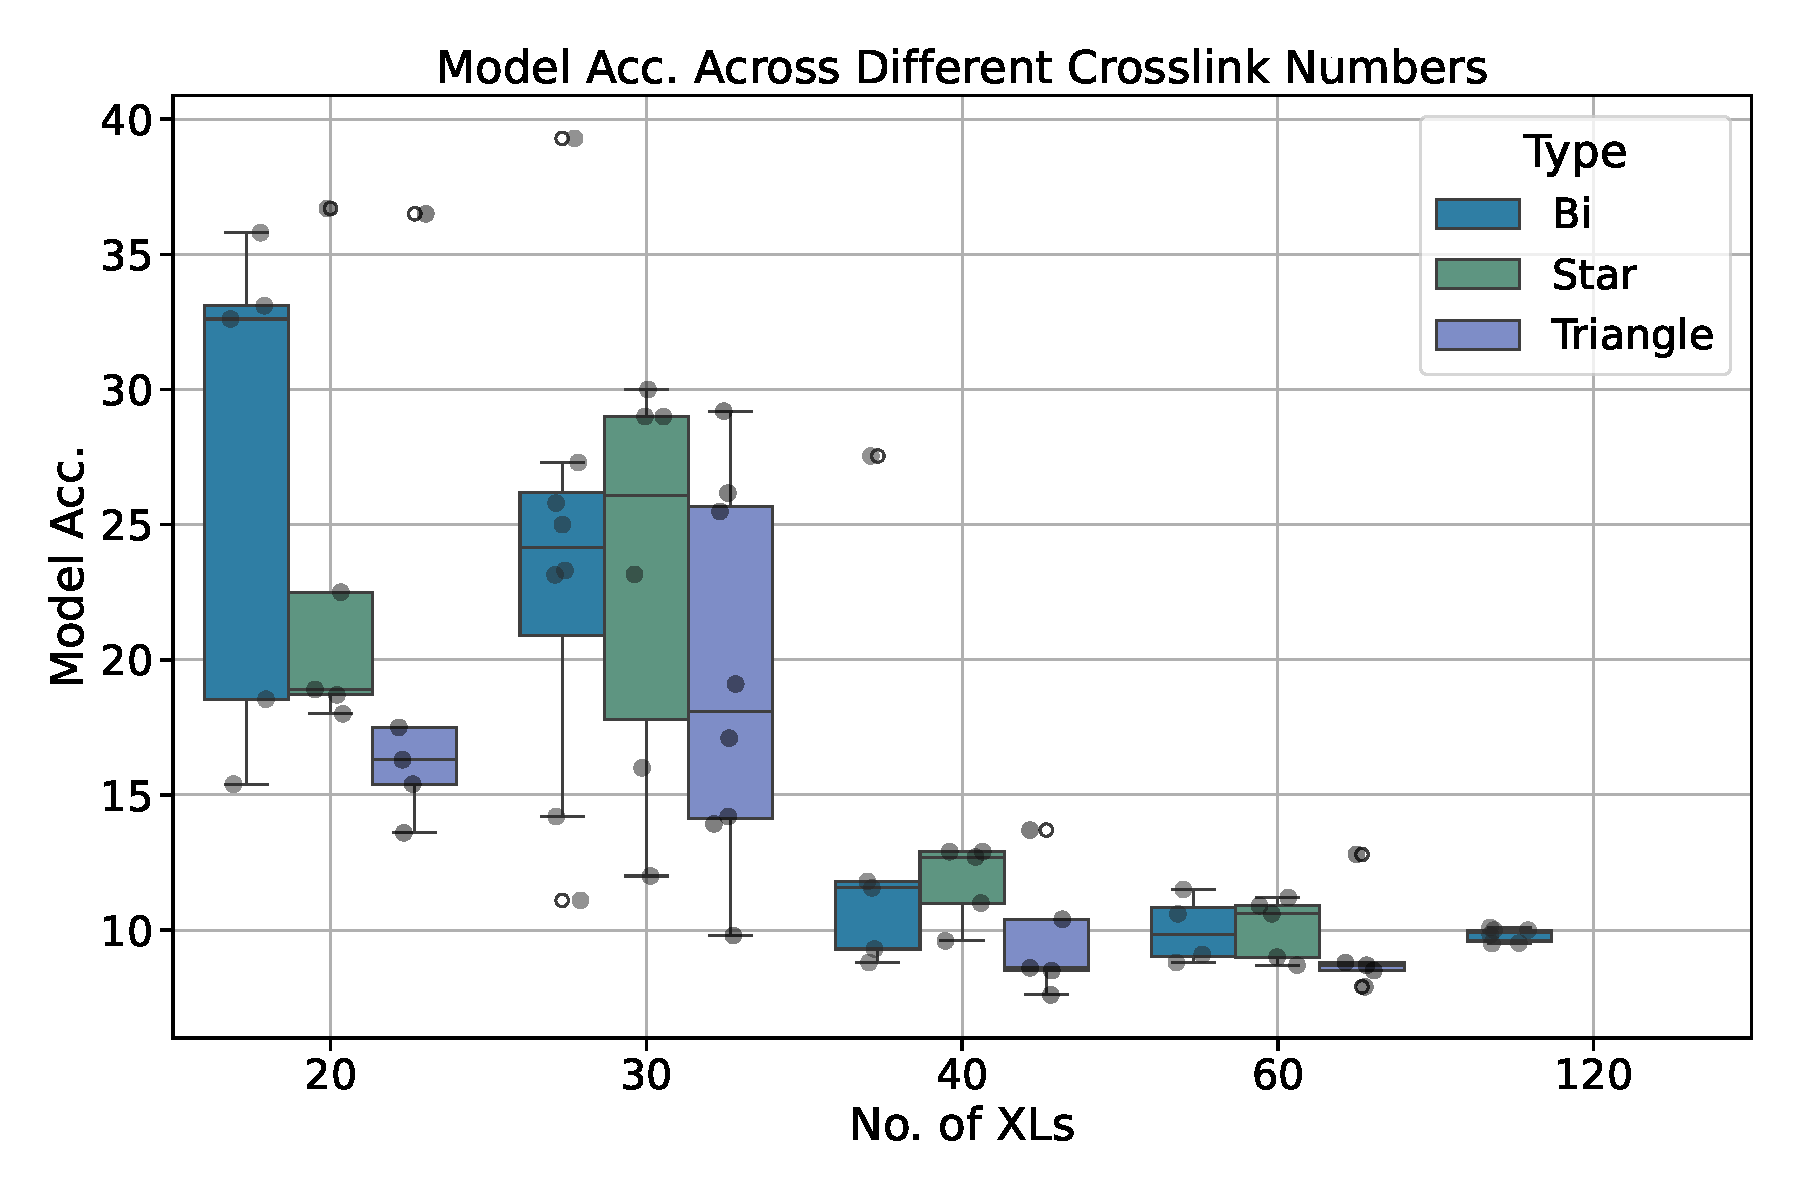
\includegraphics[width=0.45\textwidth]{test-figures/whisker_plot_model_acc.pdf}
  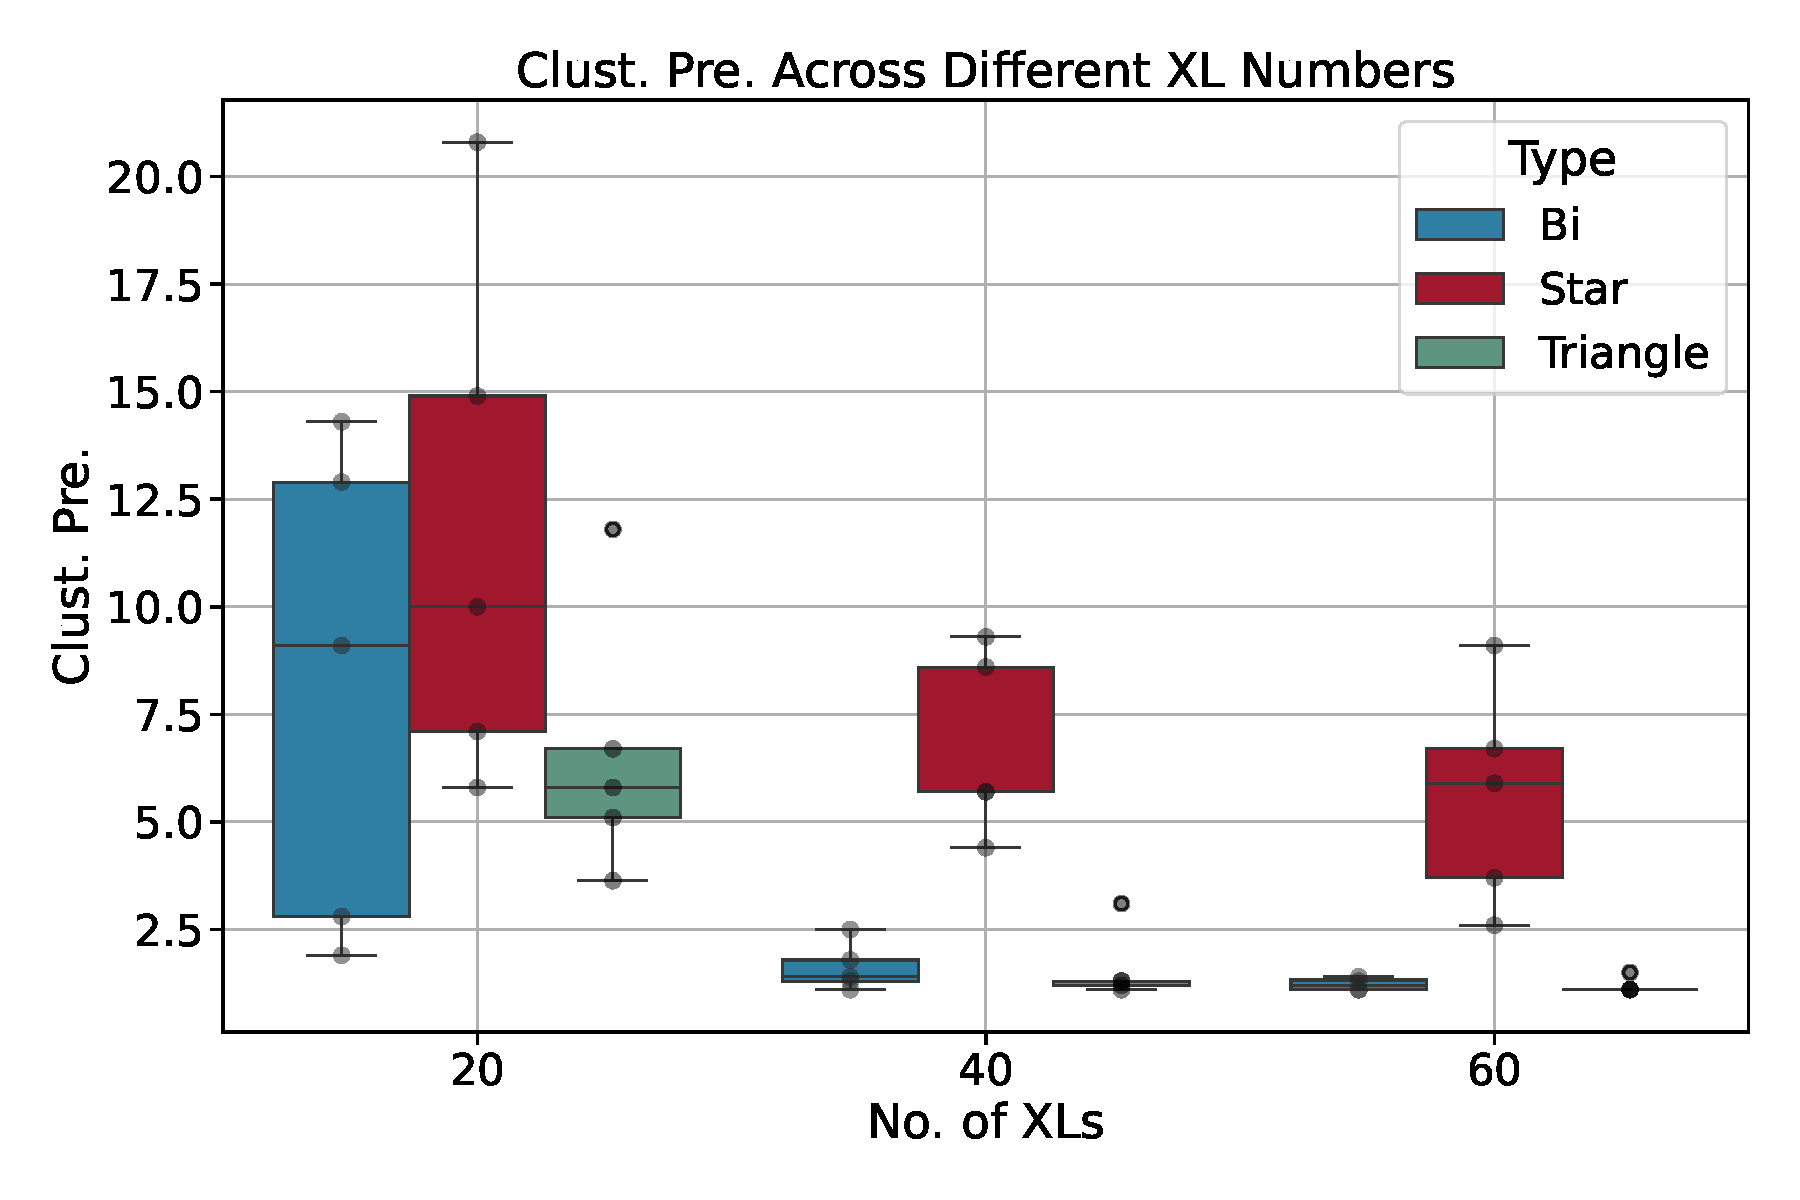
\includegraphics[width=0.45\textwidth]{test-figures/whisker_plot_clust_pre.pdf}
  \caption{Synthetic data statistics}
  \label{fig:synthetic_data_statistics}
  \end{figure}
  \end{frame}
  %
\end{document}
